\chapter{The South African energy sector}
%The Republic of South Africa (SA) is one of the most developed country in Sub-Saharan Africa and acording to the Human Development Index (HDI) it is growing constand since the 1980's, nevertheless it counts as medium developed country \cite{UNDP2014}. Also the population and energy demand is constantly growing \cite{TheWorldBank2015,Agency2015}.
The Republic of South Africa (SA) is one of the most developed countries in sub-Saharan Africa. Despite persistent poverty, its Human Development Index (HDI) has been increasing steadily since the 1980s and it is now classified as a middle-income country \cite{UNDP2015}. Population and energy demand is growing \cite{TheWorldBank2015,Agency2015}.

%SA has also one of the strongest econemys in Africa, therefore it is accounting for about \SI{30}{\percent}  of the primary energy consumption of the entire continent Africa in 2014 \cite{BP2015b}. 
South Africa also has one of the largest economies in Africa, accounting for roughly \SI{30}{\percent} of the primary energy consumption of the entire continent in 2014 \cite{BP2015b}.

\section{Primary energy consumption}

%The primary energy consumption of SA was in 2014 about \SI{1473.52}{\tera\watt\hour} \cite{BP2015b}. This consumption is mainly based on fossil energy resources. More than \SI{96}{\percent} of the primary energy consumption was in 2014 based fossil fuels and further \SI{2.8}{\percent} on nuclear. Thereby is the share on primary energy consumption predominant coming from coal. Figure \ref{PEKreis} shows the primary energy mix of SA in comparision with the worldwide primary energy mix. \cite{BP2015b}
Primary energy consumption in South Africa was \SI{1473.52}{\tera\watt\hour} in 2014 \cite{BP2015b}, of which more than \SI{96}{\percent} was in the form of fossil fuels, predominantly coal. Figure \ref{PEKreis} shows the primary energy mix\footnote{excl. biomass and waste} of SA in comparision with the global primary energy mix \cite{BP2015b}.

\begin{figure}[htbp]
        \centering                
        \begin{subfigure}[b]{0.45\textwidth}
                \centering
                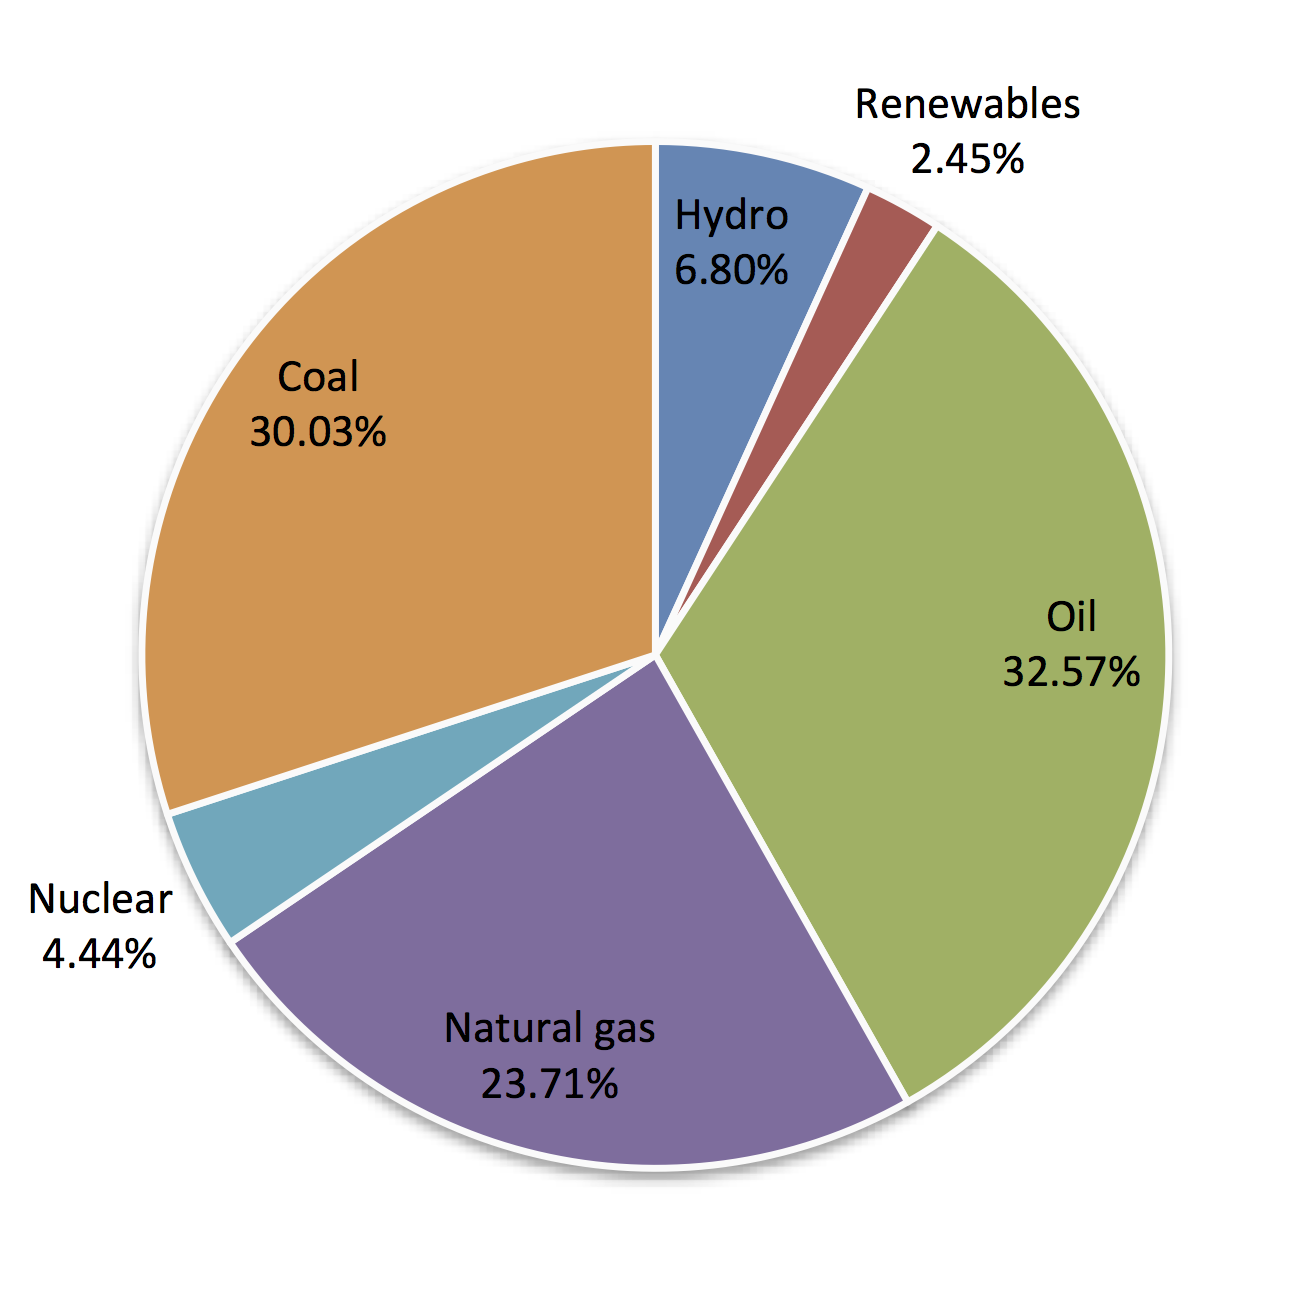
\includegraphics[width=1\textwidth]{FIG/PrimWorld}
                \caption{Global primary energy consumption.}\label{PrimWorld}
        \end{subfigure}
        ~
        \begin{subfigure}[b]{0.45\textwidth}
                \centering
                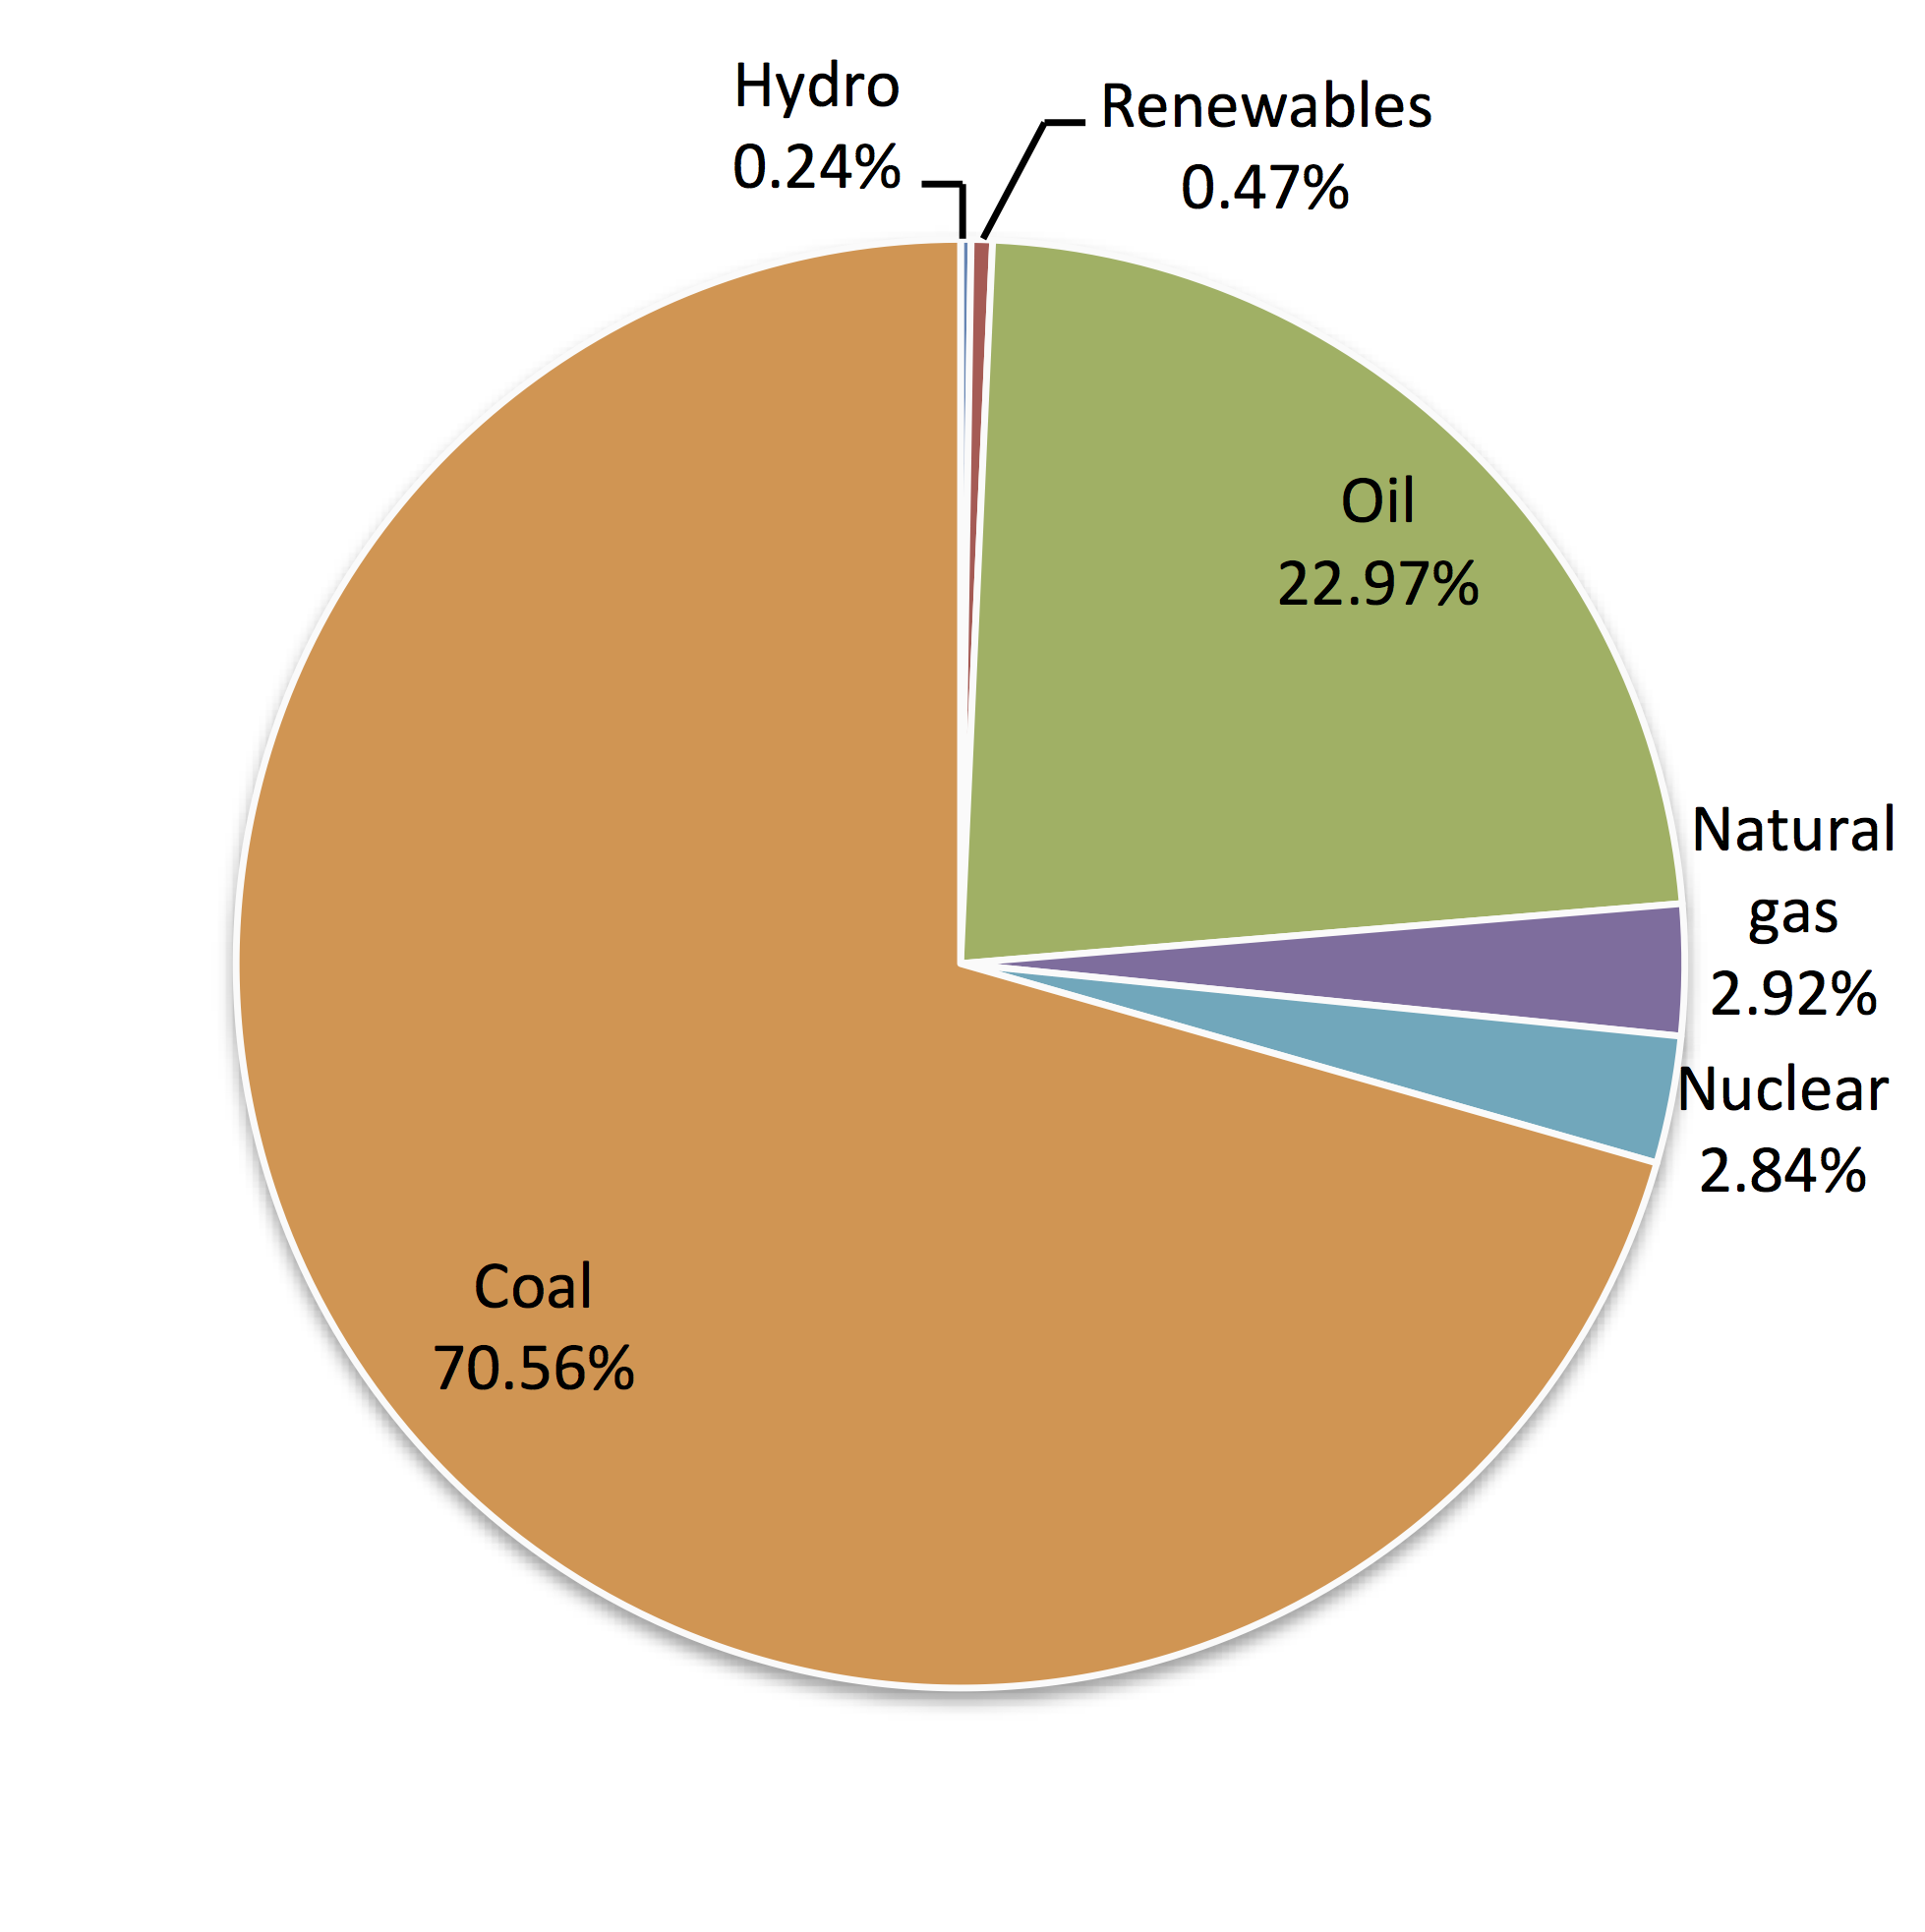
\includegraphics[width=1\textwidth]{FIG/PrimSA}
                \caption{Primary energy consumption in SA.}\label{PrimSA}
        \end{subfigure}
\caption[Comparision of primary energy consumption by fuel in 2014.]{Comparision of primary energy consumption by fuel in 2014 \cite{BP2015b}.}\label{PEKreis}
\end{figure}
%It can be seen that coal is with about 71~\% the main primary energy source. Also crude oil (\SI{23}{\percent}) is a very important energy source for SA. Therefor is the primary energy consumption from renewable energies in SA just about \SI{0.7}{\percent}. Comparing to this, the global share of  renewable primary energy consumption was about \SI{9.3}{\percent} in 2015. But it must be said that the share on renewable energy growth almost five times from 2013 to 2014. \cite{BP2015b}
Crude oil (\SI{23}{\percent}) is also a very important energy source for South Africa. The primary energy delivered by renewable sources is only \SI{0.7}{\percent}. Compare this to its share globally, which was \SI{9.3}{\percent} in 2015. Growth rates for renewable energy have been high, however, growing almost five times from 2013 to 2014 \cite{BP2015b}.

%Figure \ref{PrimEnergyDevelopment} shows the growing South African primary energy consumption. Between 1965 and 2014 the annual primary energy consumption in SA has risen from \SI{351.96}{\tera\watt\hour} up to \SI{1473.52}{\tera\watt\hour}. Consequently a avarage anual growing rate in primary energy consumption in SA of \SI{8.5}{\percent} in the past half century. \cite{BP2015c}
Overall primary energy consumption continues to grow (Figure \ref{PrimEnergyDevelopment}). Between 1965 and 2014, annual primary energy consumption rose from \SI{351.96}{\tera\watt\hour} to \SI{1473.52}{\tera\watt\hour}, corresponding to an average annual growth rate of \SI{8.5}{\percent} in the past half century \cite{BP2015c}.

\begin{figure}[htbp]  
\centering
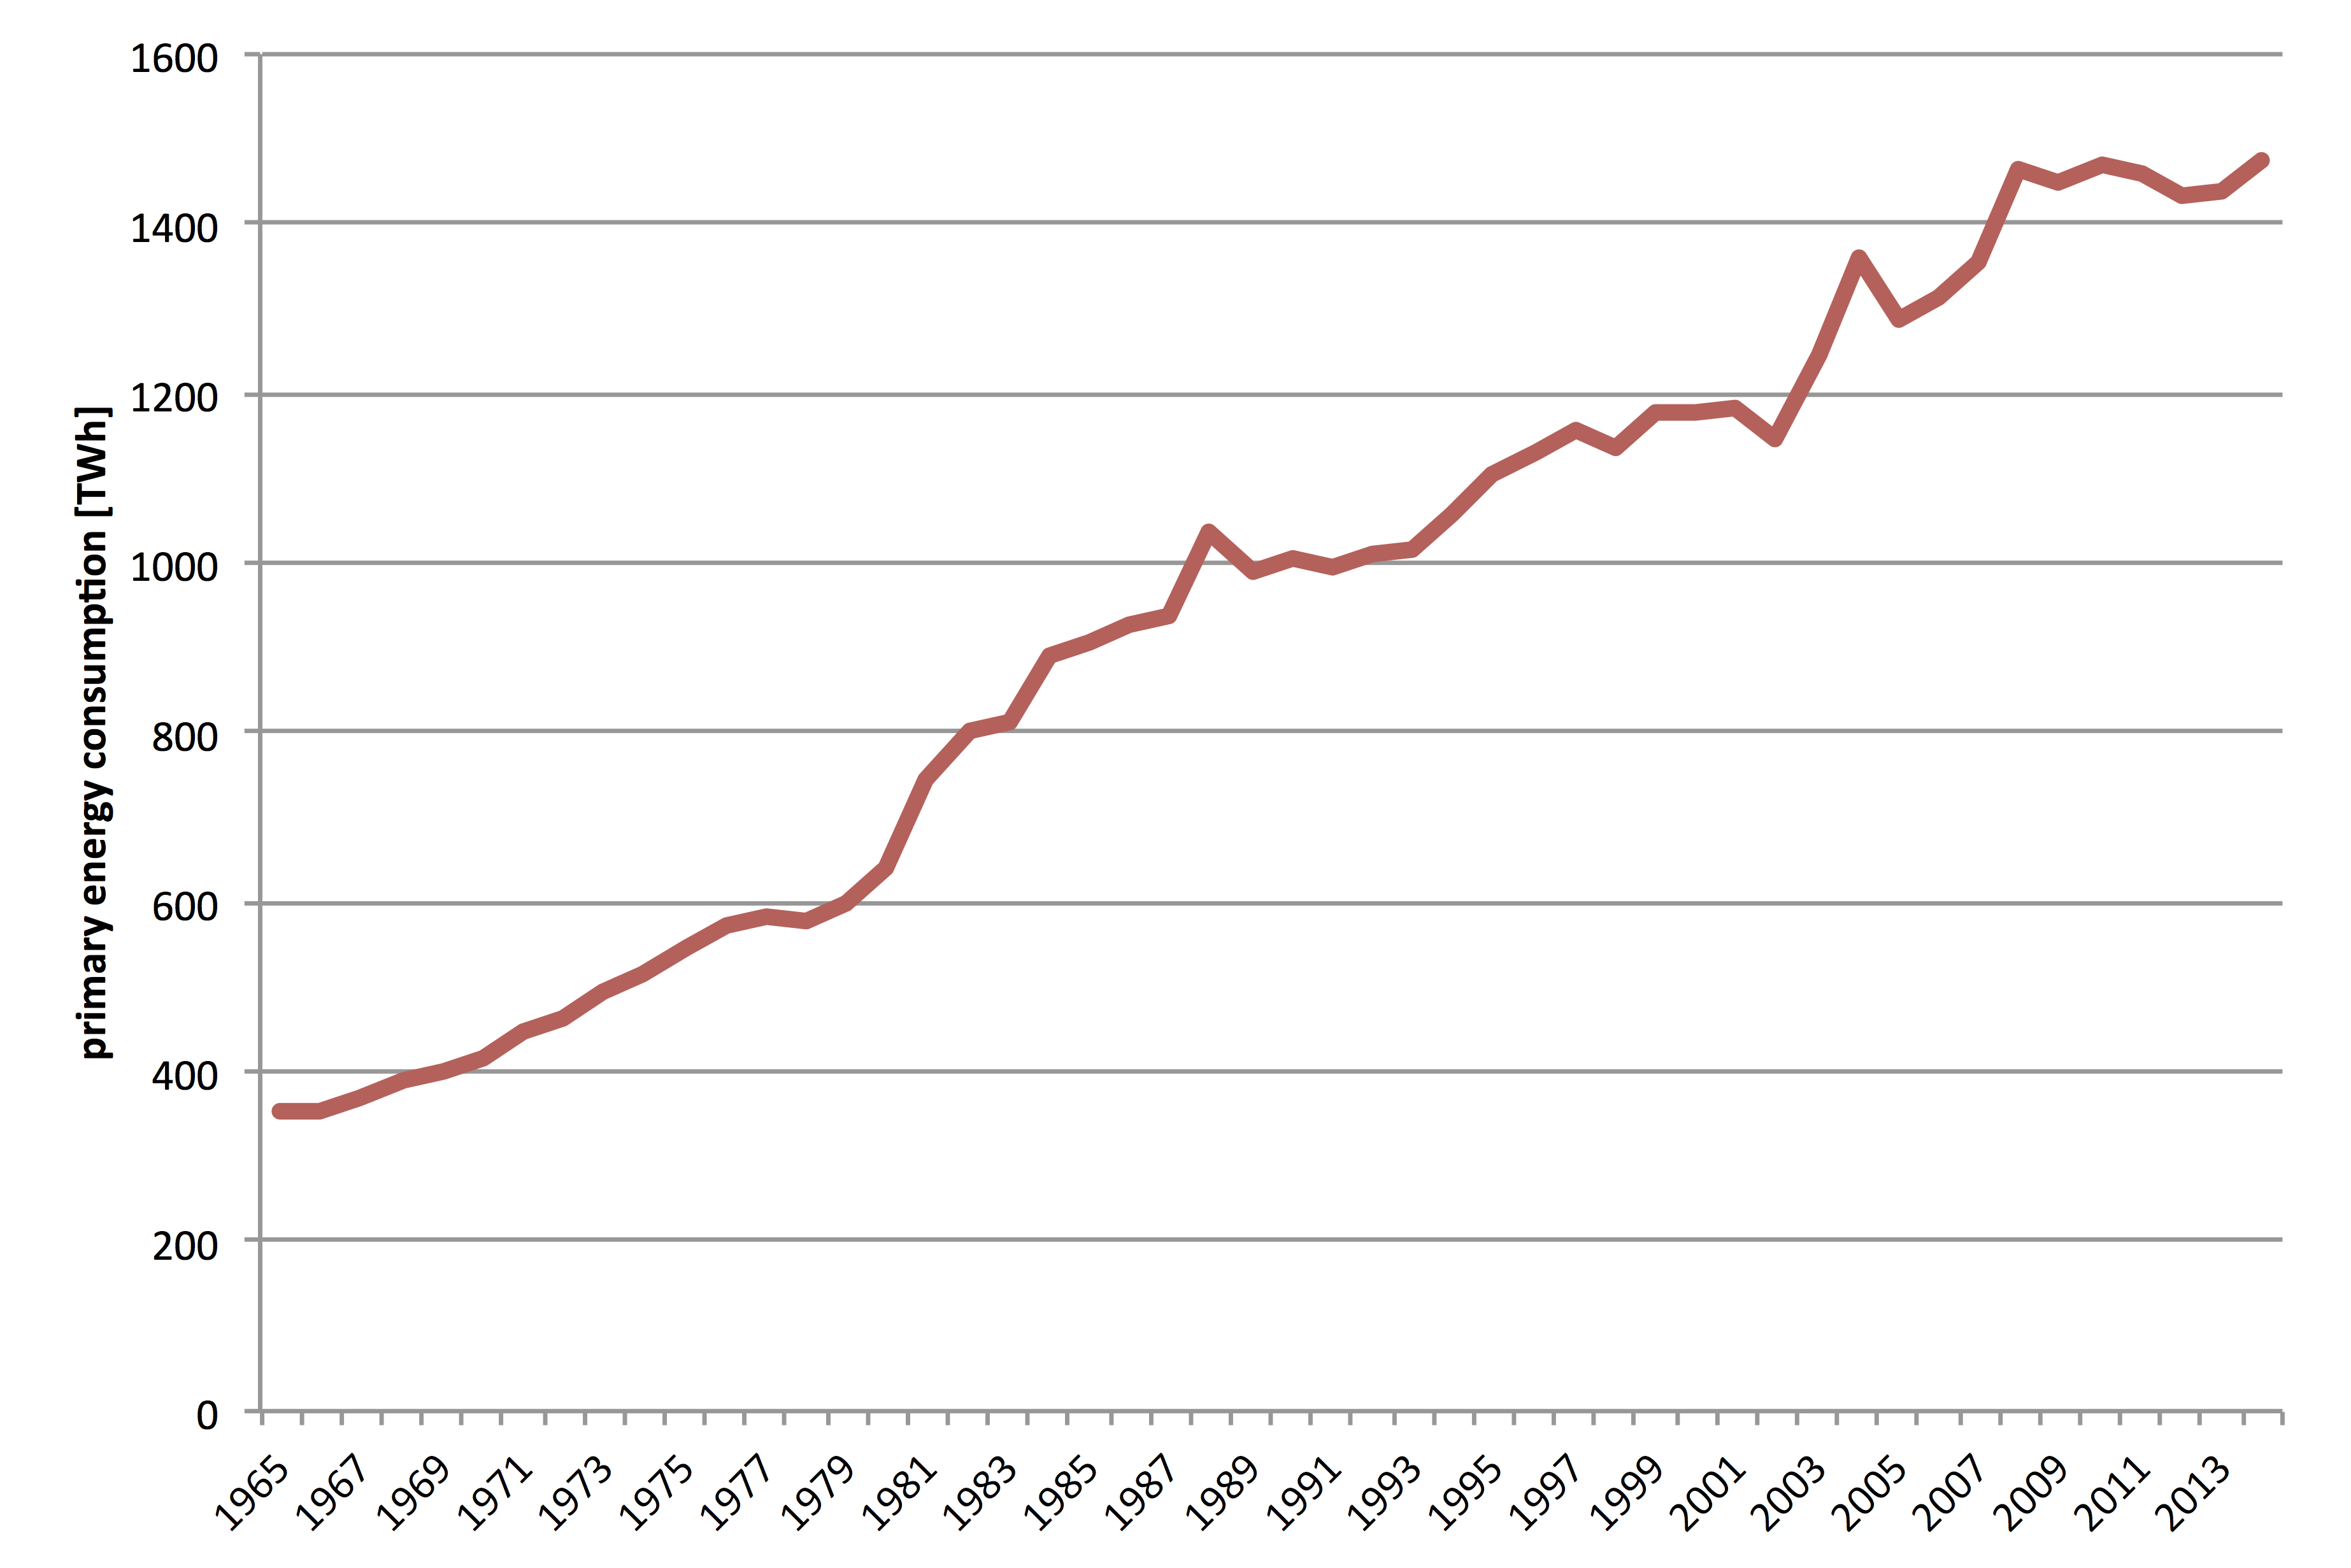
\includegraphics[width=1\linewidth]{FIG/PrimEnergyDevelopment}
\caption[Evolution of primary energy consumption in South Africa.]{Evolution of primary energy consumption in South Africa \cite{BP2015c}.}\label{PrimEnergyDevelopment}
\end{figure}
%The spread in consumption of primary energy is defined by three major consumption groups, namly the industry sector with about \SI{34.9}{\percent}, the transport sector which consumes about \SI{28.6}{\percent} and other sectors with about \SI{36.5}{\percent}, which includes agriculture, commerce and public services, residential and non-specified consumers \cite{DepartmentofEnergy2012}. So it can be said that the sectors industy and transport are the main energy consumer in SA. 
The largest consumers of primary energy by sector are industry (\SI{34.9}{\percent}) and transport (\SI{28.6}{\percent}), with the remainder (\SI{36.5}{\percent}) owing to agriculture, commerce and public services, residential and non-specified consumers \cite{DepartmentofEnergy2012}.

\pagebreak
\section{Electricity supply and demand} \label{ElectricitySA}
%The electricity market in SA is regulated by the National Energy Regulator of South Africa (NERSA) in terms of the National Energy Regulatory Act from 2004. NERSA's area of responsibility includes the national grid codes, licences, provides, regulations of tariff increases and more. \cite{Eskom2015a}
The electricity market is regulated by the National Energy Regulator of South Africa (NERSA) according to the terms of the National Energy Regulatory Act of 2004. NERSA's areas of responsibility include national grid codes, licencing, and tariff regulation \cite{Eskom2015a}.

%SA has a fully state-owned and vertically integrated electricity supplier named Eskom (Eskom Holdings SOC Ltd.). Eskom supplies approximately \SI{95}{\percent} of SA's electricity and more than \SI{45}{\percent} of Africa \cite{EskomGenerationDivision2014}. In 2014 SA has a \SI{1.1}{\percent} share of the worldwide electricity consumption with a gross electricity output of \SI{252.6}{\tera\watt\hour} \cite{BP2015c}. \SI{92.6}{\percent} of SA's primary energy consumption for electricity generation was based on coal fired power plants in 2013 and further \SI{5.5}{\percent} came by nuclear power plant \cite{Agency2015}. Therefore was Eskom in 2009 with \SI{215.91}{\mega\tonne}~CO\textsubscript{2} also worldwide number five of the power companies with the highest CO\textsubscript{2} emissions \cite{CARMA2015}.
South Africa's fully state-owned and vertically-integrated electricity supplier, Eskom Holdings SOC Ltd., supplies \SI{95}{\percent} of the country's electricity and more than \SI{45}{\percent} of Africa's \cite{EskomGenerationDivision2014}. In 2014, South Africa had \SI{1.1}{\percent} share of worldwide electricity consumption, with gross electricity output of \SI{252.6}{\tera\watt\hour} \cite{BP2015c}.
The largest, overwhelming portion of primary energy for electricity generation was due to coal-fired power plants. In 2009, Eskom had the fifth highest CO\textsubscript{2} emissions in the world among electrical utilities, at \SI{215.91}{\mega\tonne}~CO\textsubscript{2} \cite{CARMA2015}.

%Figure~\ref{Electr} compares the South African and worldwide primary energy consumption for electricity generation in 2013. As it is shown, besides coal and nuclear based power generation makes just hydroelectric generation any significant part. \cite{Agency2015}

Figure~\ref{Electr} compares the South African and worldwide primary energy consumption for electricity generation in 2013. Beyond coal and nuclear energy, only hydroelectric is a significant contributor to electricity generation \cite{Agency2015}.

\begin{figure}[!htbp]
        \centering                
        \begin{subfigure}[b]{0.45\textwidth}
                \centering
                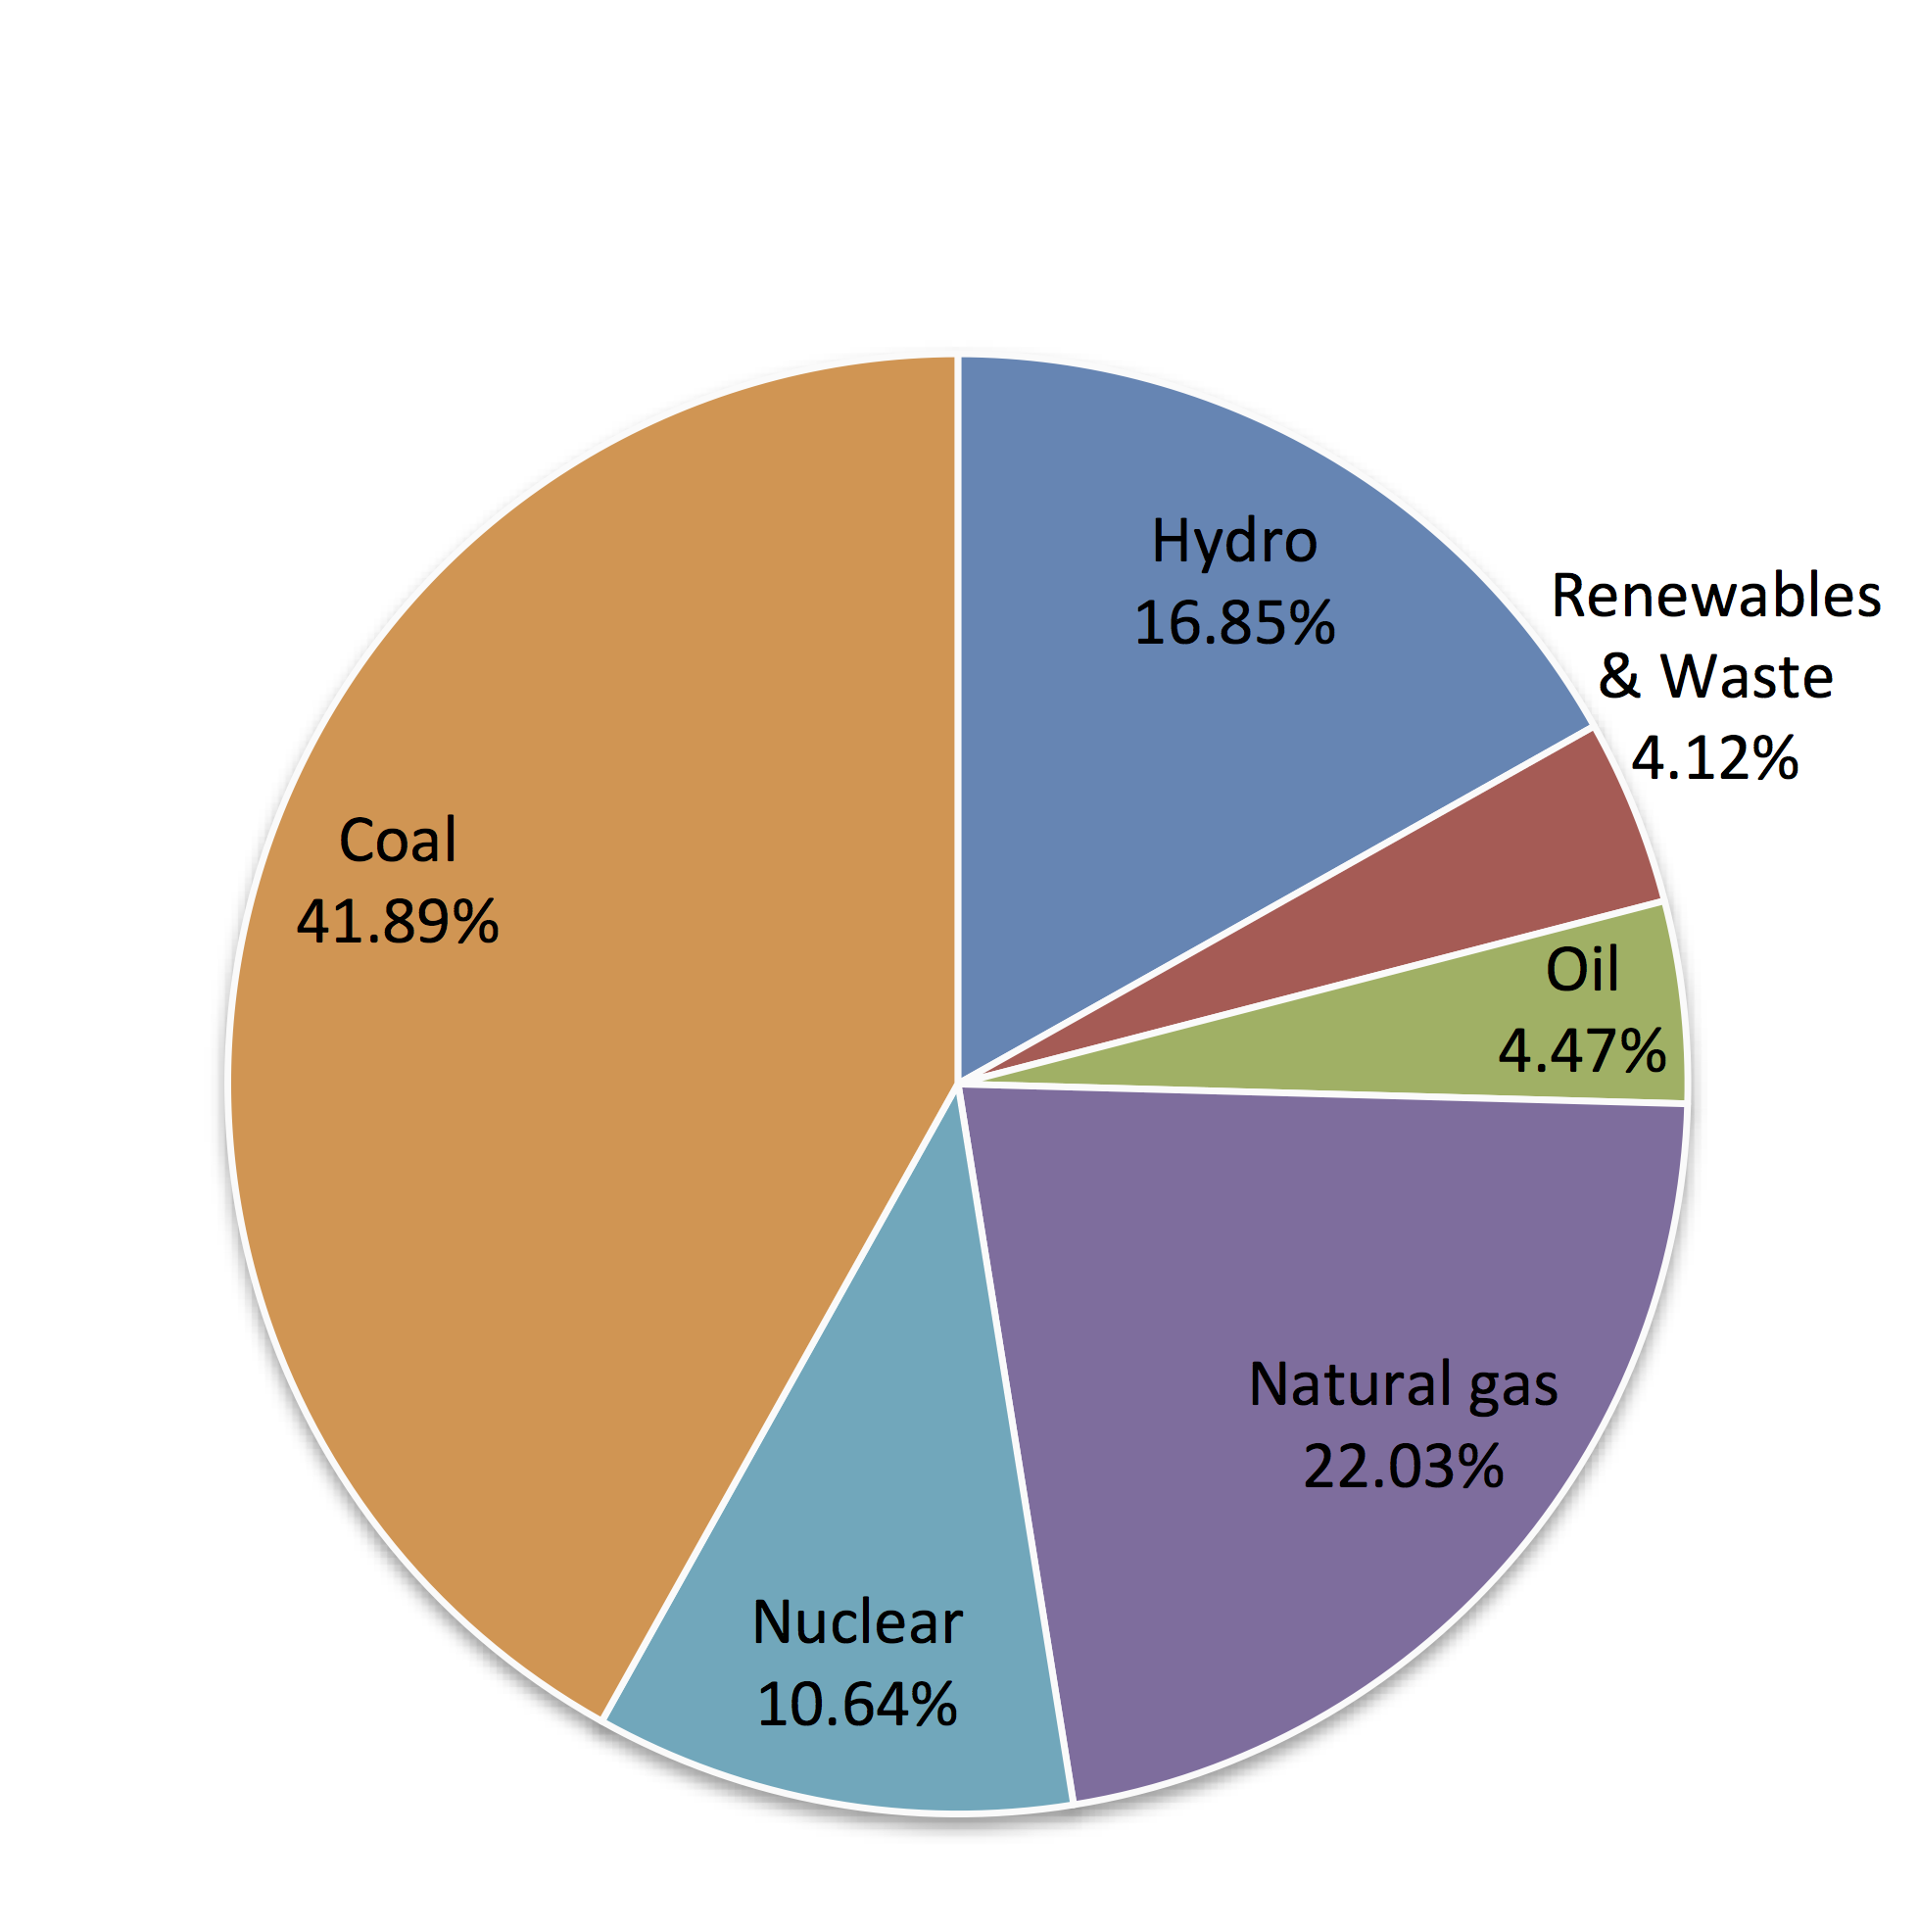
\includegraphics[width=1\textwidth]{FIG/ElectrWorld}
%                \caption{World's allocation of primary energy consumption for electricity generation.}\label{ElectrWorld}
                \caption{Primary energy consumption for electricity generation (world).}\label{ElectrWorld}
        \end{subfigure}
        ~
        \begin{subfigure}[b]{0.45\textwidth}
                \centering
                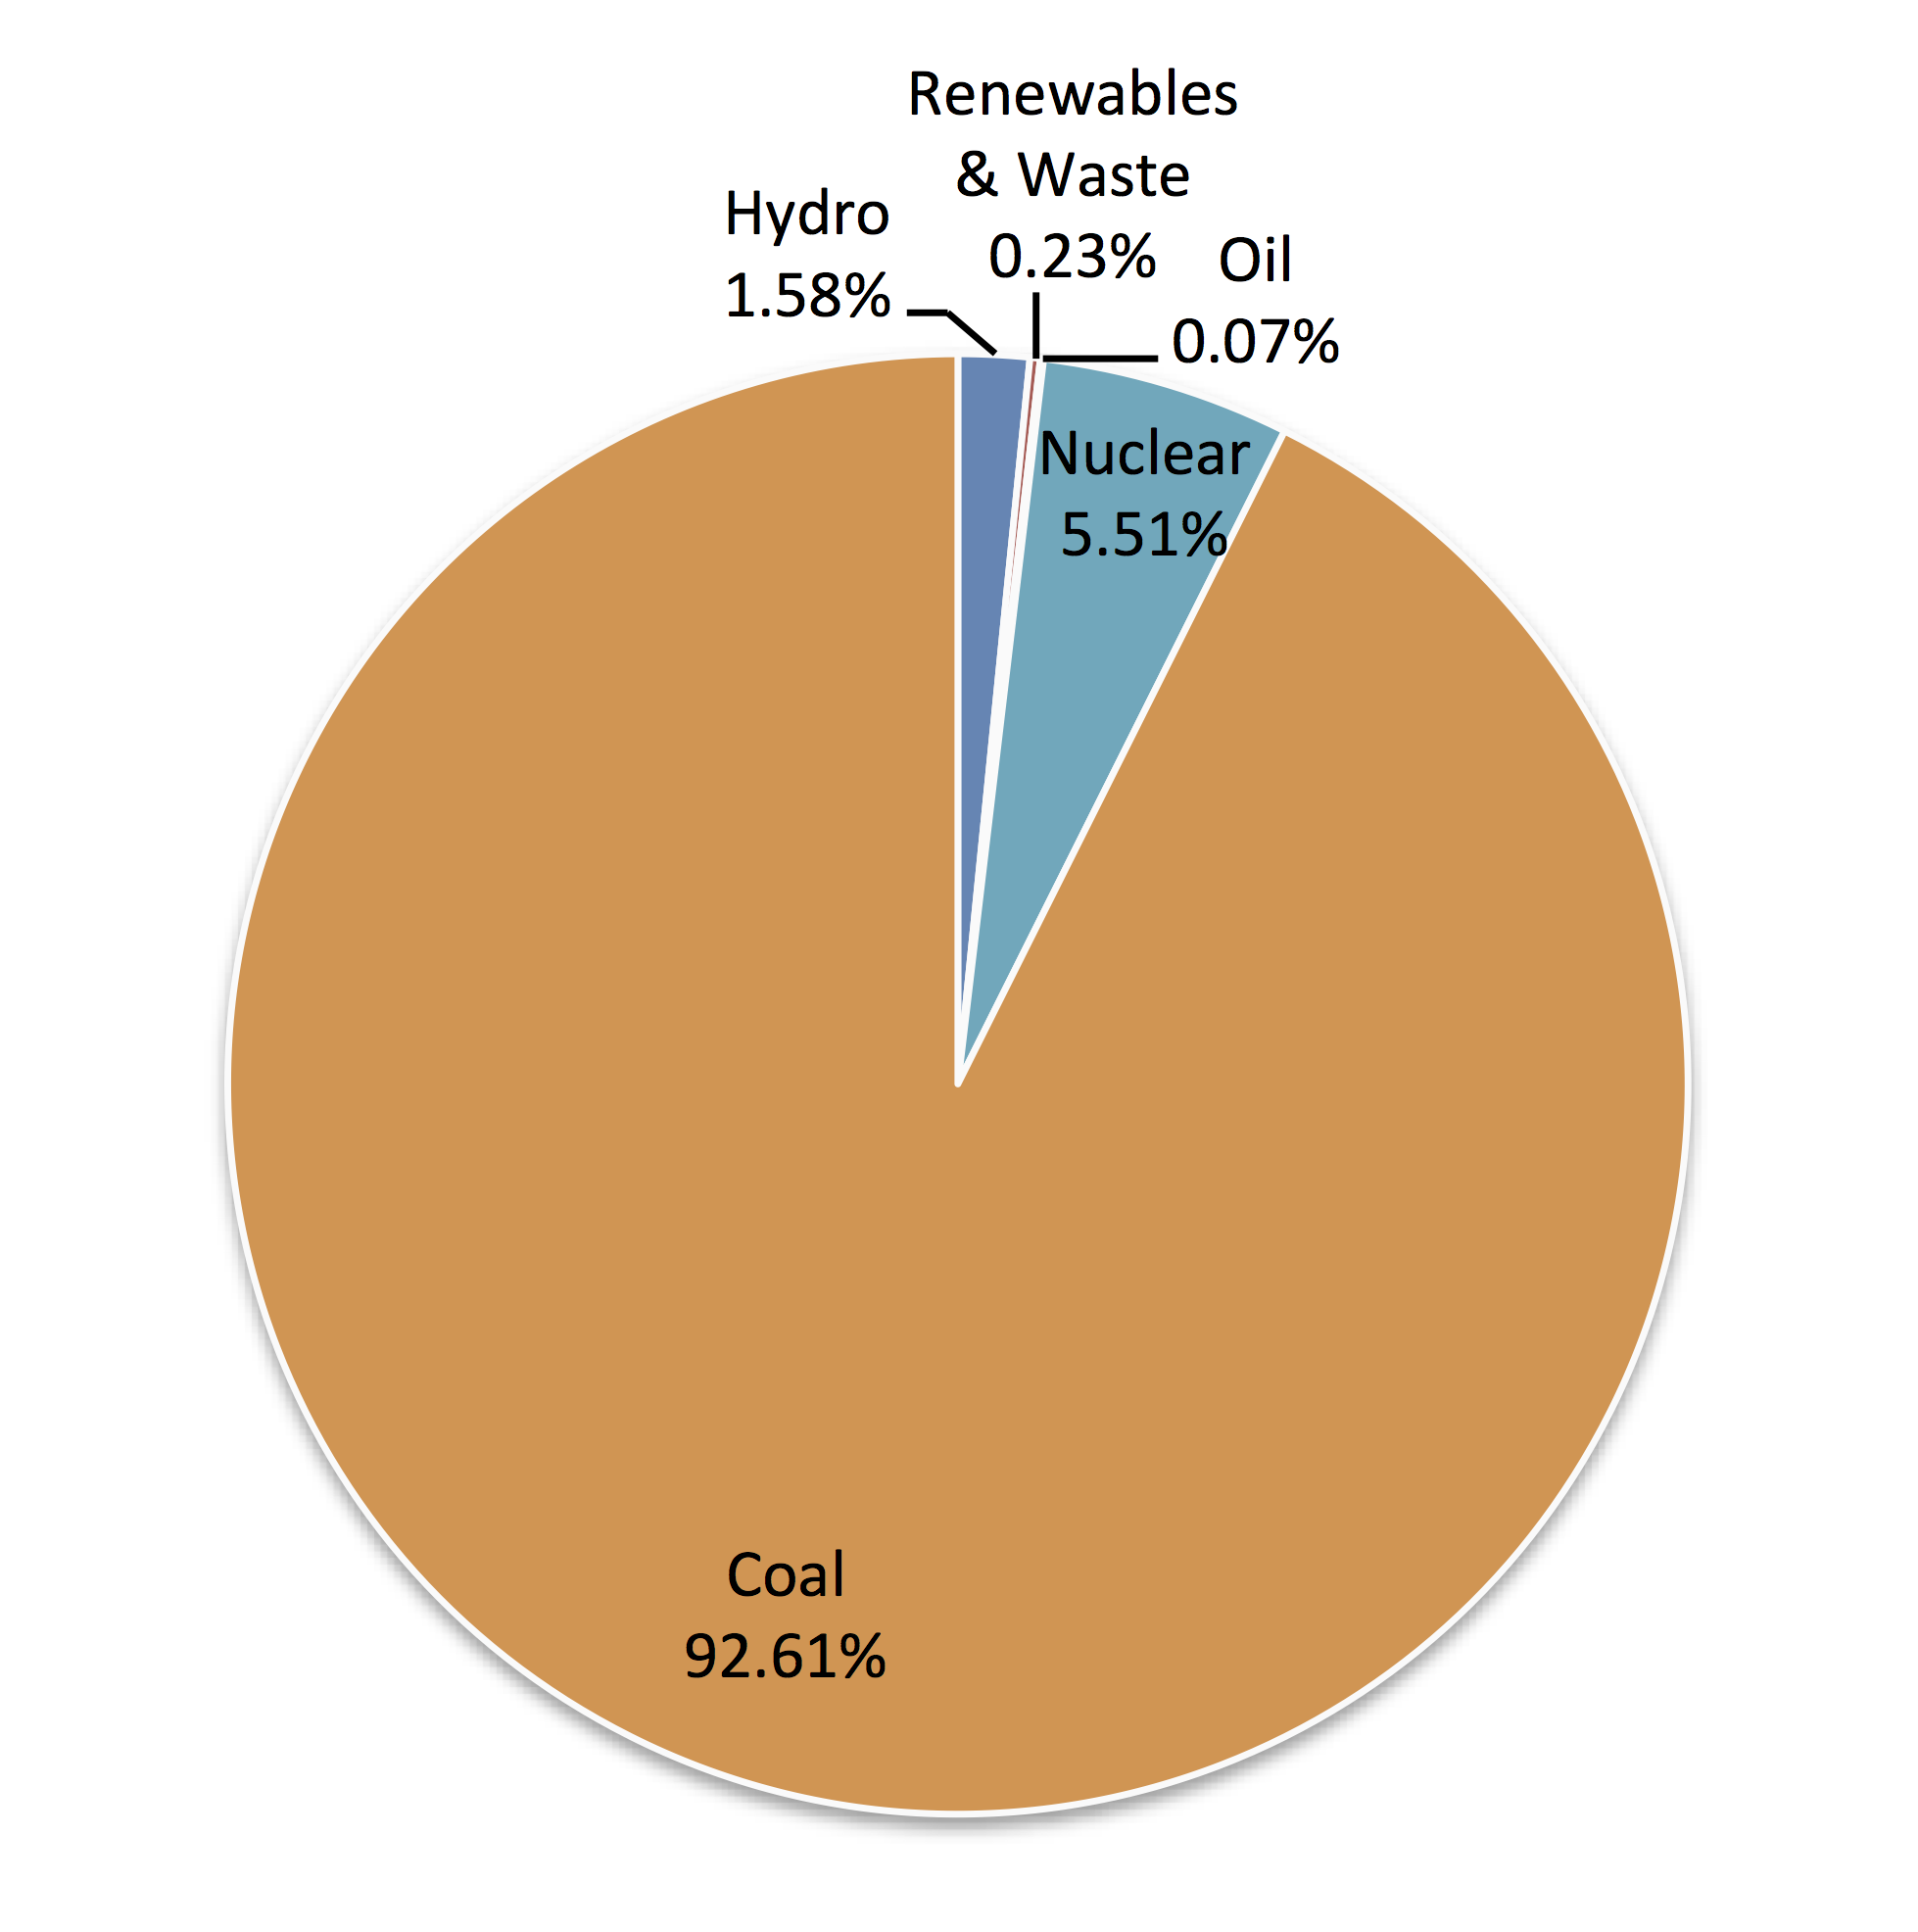
\includegraphics[width=1\textwidth]{FIG/ElectrSA}
                \caption{Primary energy consumption for electricity generation in South Africa.}\label{ElectrSA}
        \end{subfigure}
\caption[Comparision of primary energy consumption for electricity generation by fuel in 2013.]{Comparision of primary energy consumption for electricity generation by fuel in 2013 \cite{Agency2015}.}\label{Electr}
\end{figure}
%As mentioned in 2014 the gross electricity generation was about \SI{252.58}{\tera\watt\hour} in SA. But when taking an eye on the evolution of the gross electricity generation of the last three decades in Figure~\ref{electrGross} it can be noted that the generation peaked in 2007 with \SI{263,48}{\tera\watt\hour}. \cite{BP2015c} 

\begin{figure}[htbp]  
\centering
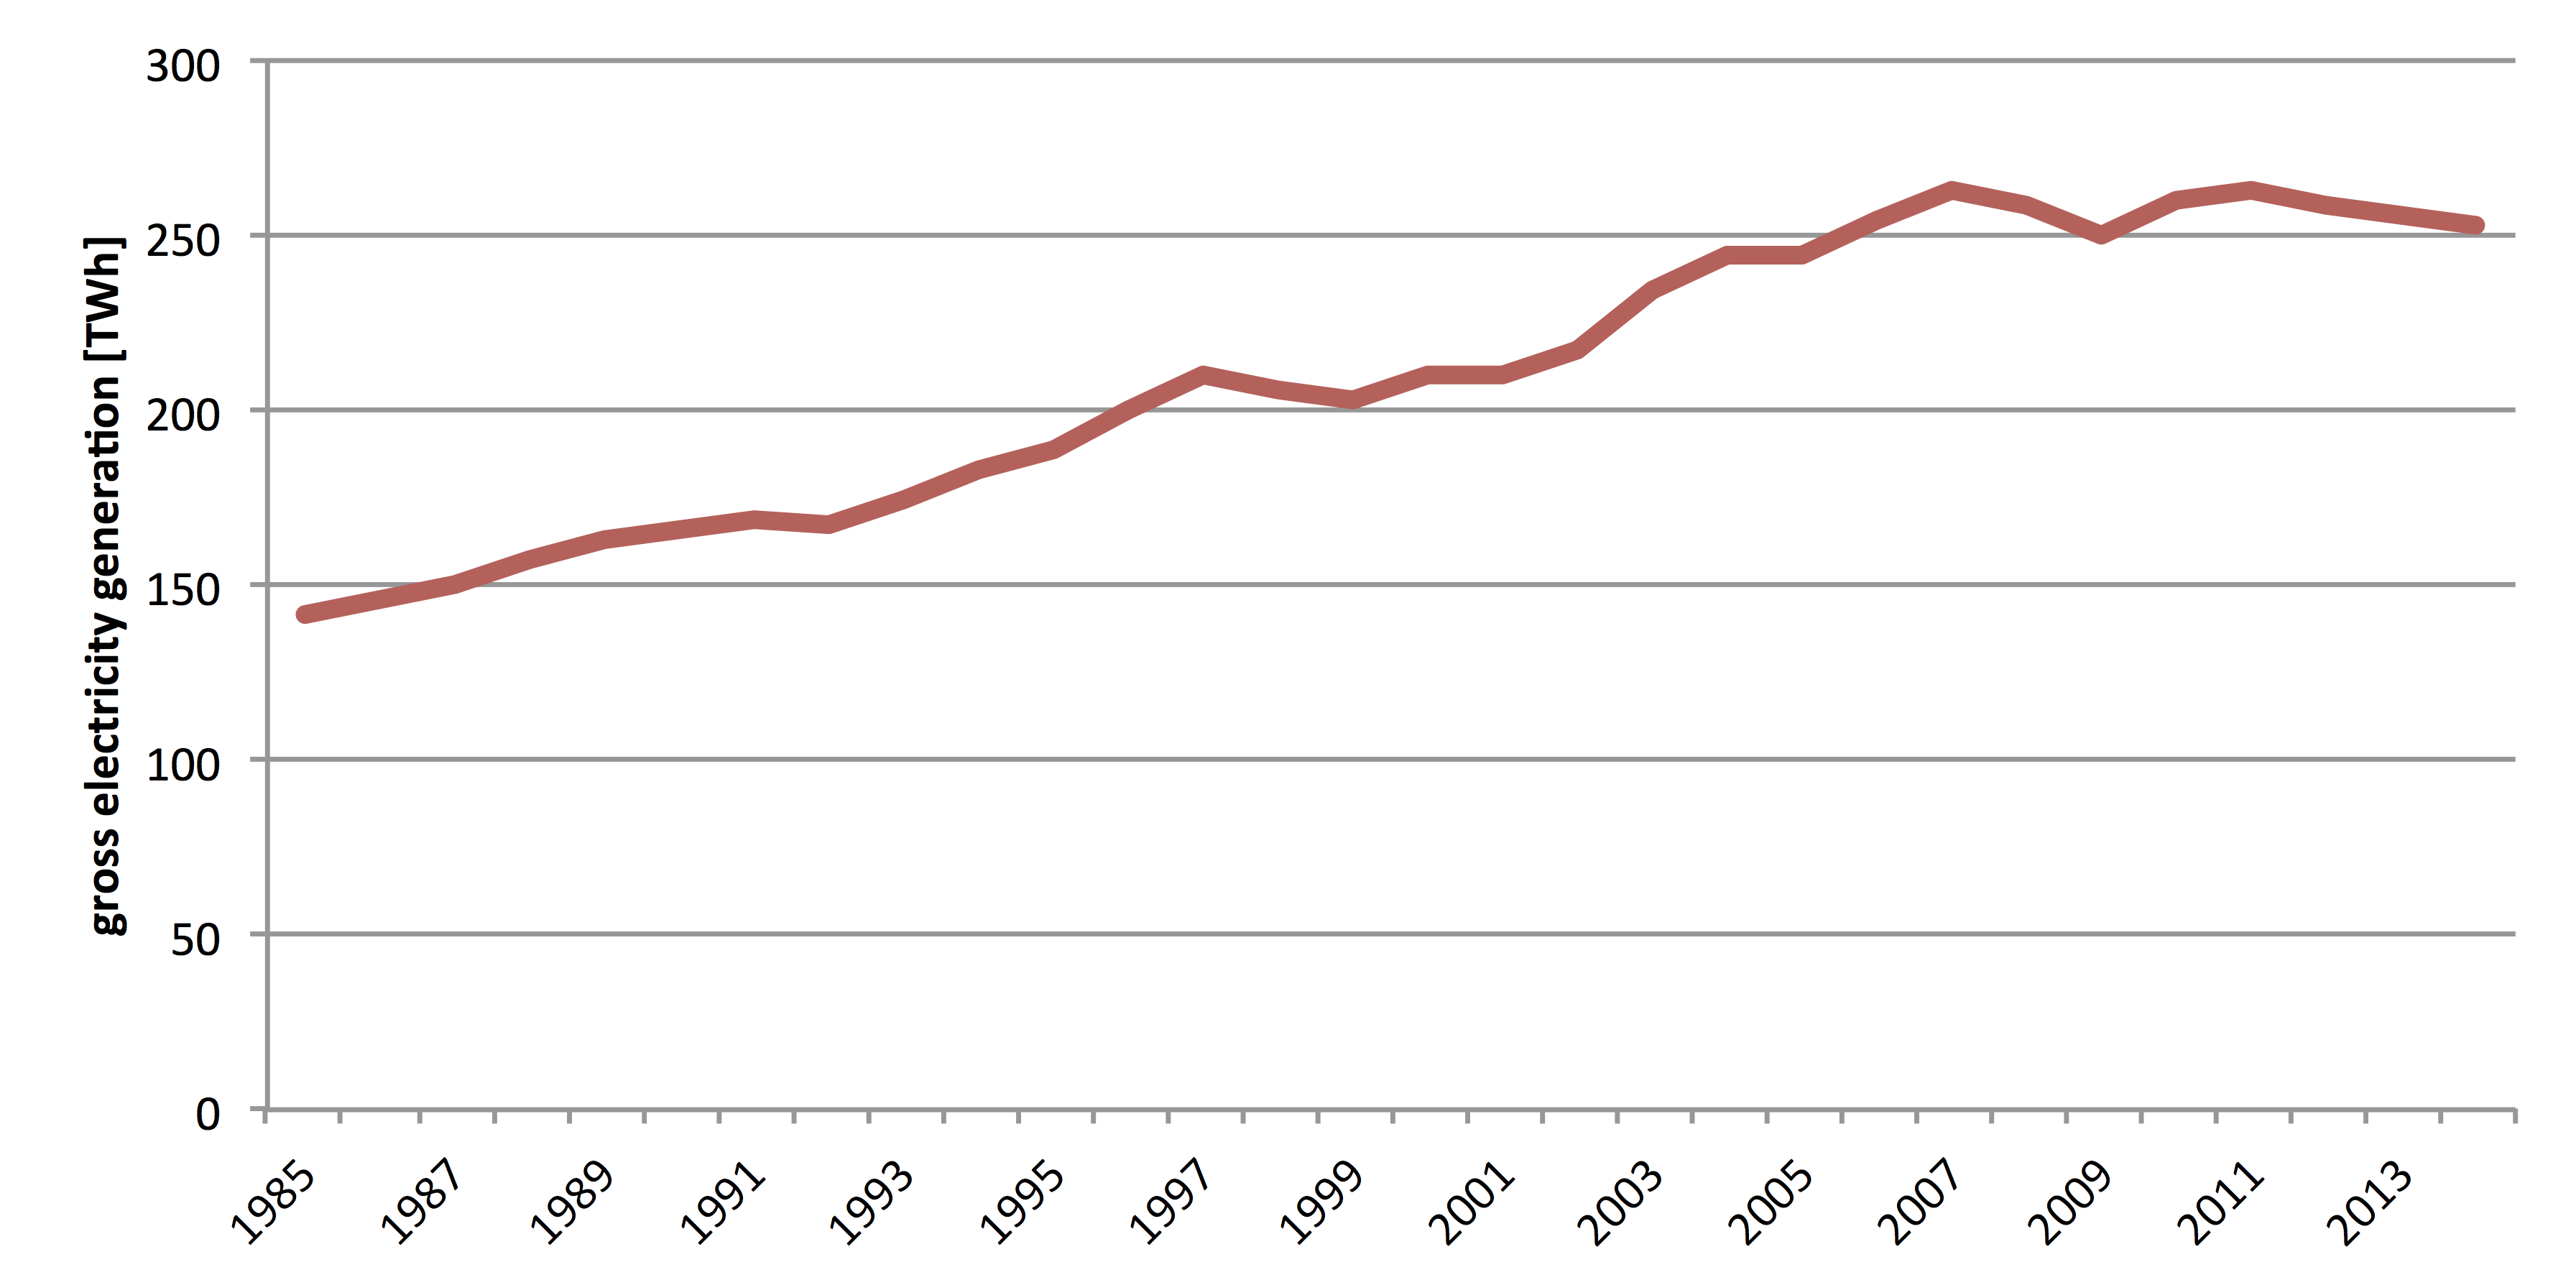
\includegraphics[width=1\linewidth]{FIG/electrGross}
\caption[Evolution of gross electricity generation in SA.]{Evolution of gross electricity generation in SA \cite{BP2015c}.}\label{electrGross}
\end{figure}
Consider the evolution of electricity generation over the last three decades (Figure~\ref{electrGross}). Total electrical energy generated peaked in 2007 at \SI{263,48}{\tera\watt\hour}. \cite{BP2015c} 

%The leak on growth momentum of gross electricity generation in SA after the global financial crisis in 2009 is not leading from decreasing request in demand, but more from a power plant maintainence behind schedule and investment backlog. The delayed maintainence schedule was a results from Eskom’s “keeping the lights on” philosophy what they are calling nowadays a "not sustainable approach" \cite{Eskom2014}. Eskom’s base load fleet has a average age of about 34 years with a plant availability of about \SI{73}{\percent} \cite{Eskom2015c}. This facts be associated with the rising annual unplanned capability loss factor (UCLF) of Eskom’s power plant fleet. Figure~\ref{UCLF} shows that the UCLF rises from 2008/09 on significantly. In 2014/15 the UCLF reached their maximum of \SI{15.22}{\percent}. The rising UCLF comes in hand with implementing of “load shedding” by Eskom in 2008, which is a planned rolling blackouts based on a schedule in order to protect the power system from a total blackout \cite{Eskom2015d}. Eskom implemted a load shedding schedule in four stages, wich allows Eskom at Stage 4 to dropping of up to \SI{4000}{\mega\watt} of the national load to balance electricity supply and demand. \cite{Eskom2015e}
The plateau in electricity production following the global financial crisis in 2009 is not the result of decreasing demand, but rather delayed plant maintenance and an infrastructure deficit. The delayed maintenance was the result of Eskom's \enquote{keeping the lights on} philosophy, which the company has since acknowledged is \enquote{not sustainable} \cite{Eskom2014}. Eskom's base load fleet has an average age of approximately 34 years, with a plant availability of about \SI{73}{\percent} \cite{Eskom2015c}. This is the principal cause of increases in unplanned capability loss factor (UCLF) (Figure~\ref{UCLF}). In 2008, Eskom implemented a load shedding scheme; this consists of planned rolling blackouts based on a schedule in order to protect the power system from a total blackout \cite{Eskom2015d}. The four-stage scheme allows Eskom to drop up to \SI{4000}{\mega\watt} of load at Stage 4 to balance electricity supply and demand \cite{Eskom2015e}.

\begin{figure}[htbp]  
\centering
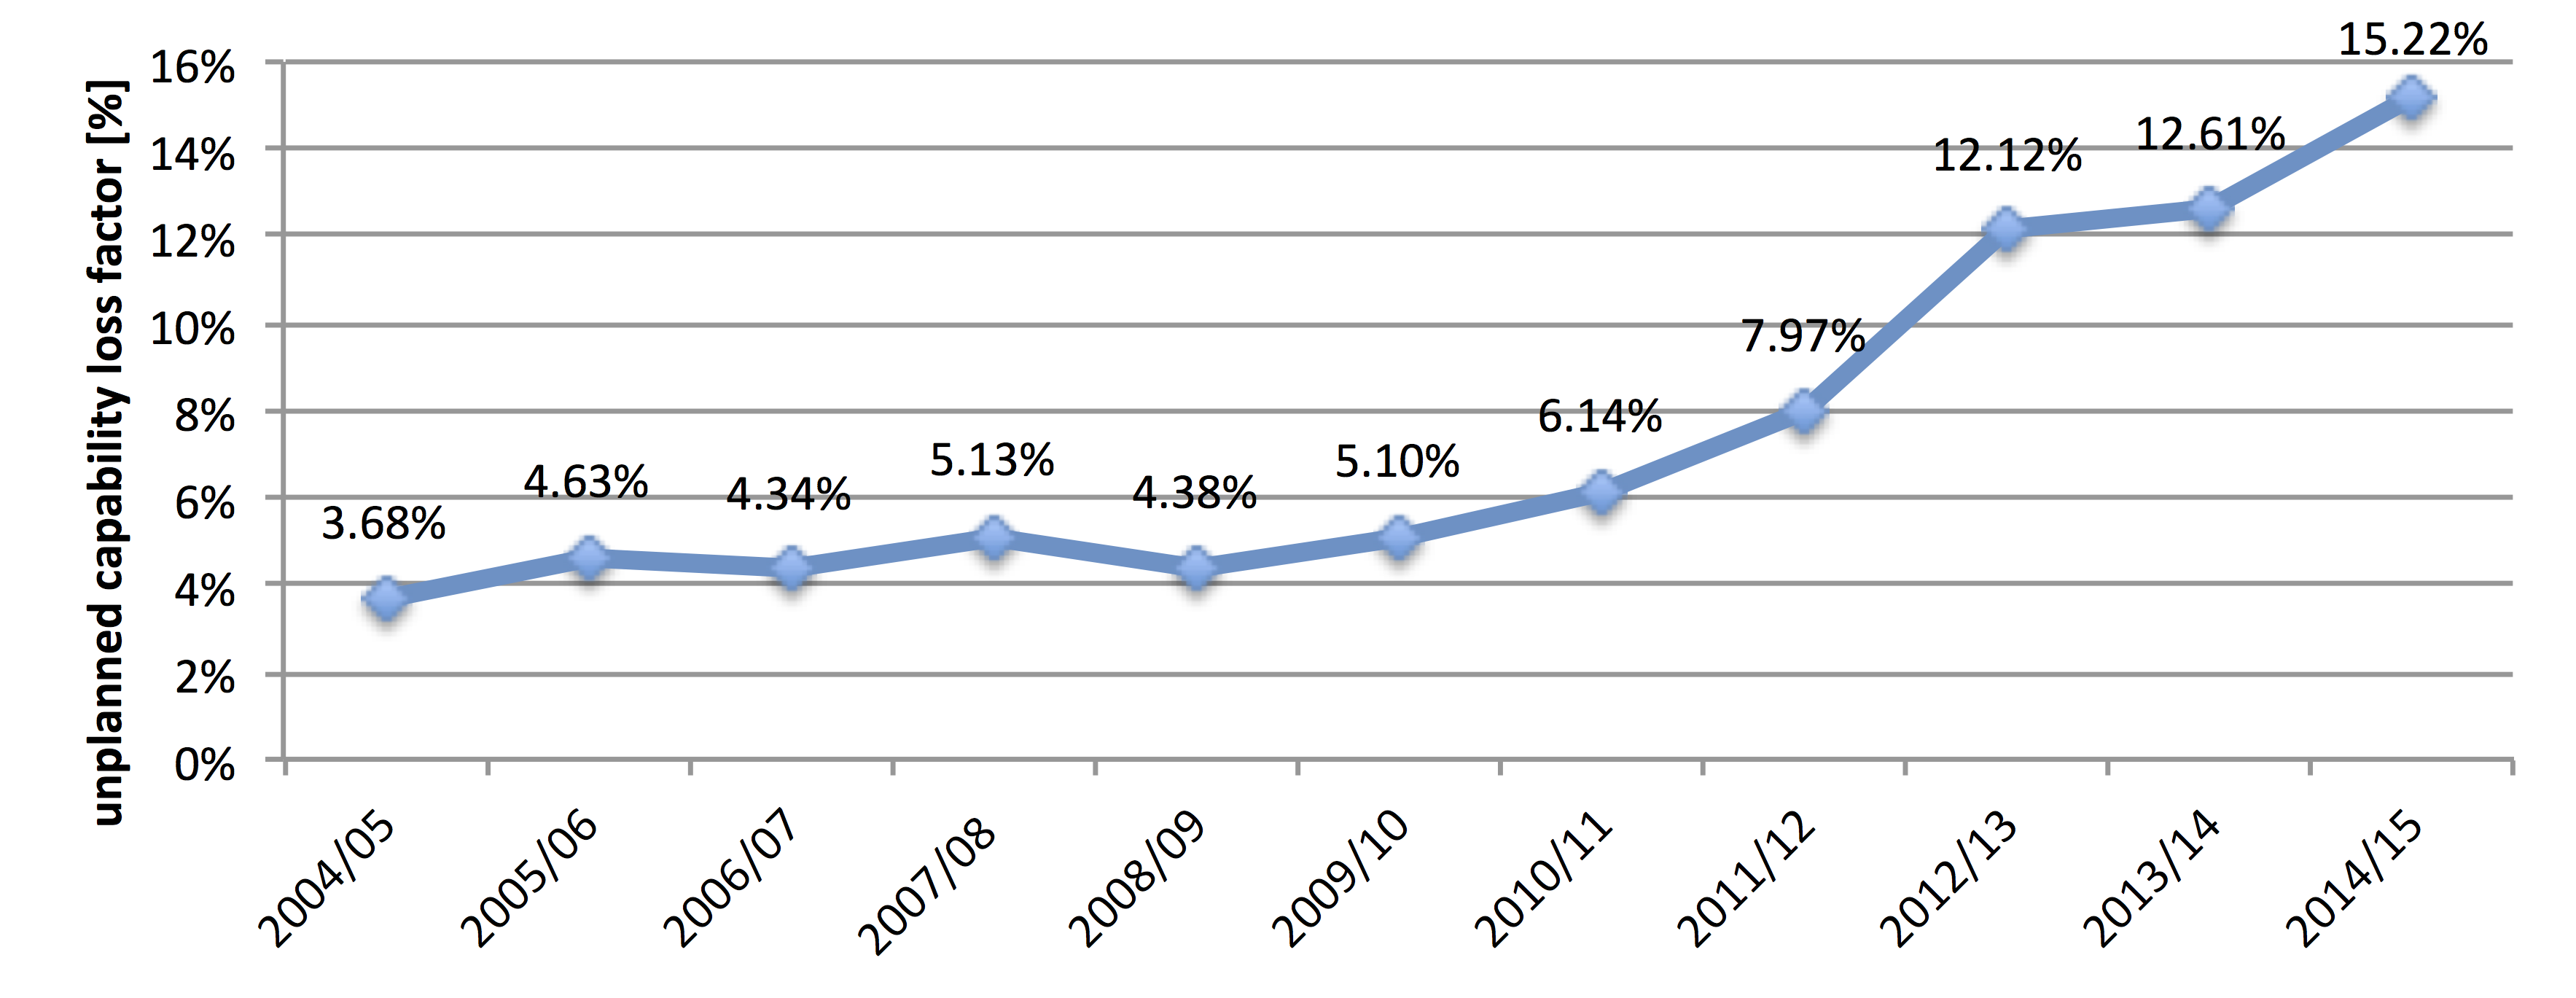
\includegraphics[width=1\linewidth]{FIG/UCLF}
\caption[Evolution of Eskom's annual unplanned capability loss factor.]{Evolution of Eskom's annual unplanned capability loss factor \cite{Eskom2015b,Eskom2015d}.}\label{UCLF}
\end{figure}

%When taking an eye on the load shedding history of the first half year of 2015 in Figure~\ref{Load_shedding} it is obviously that the capacity bottleneck is mostly in the daytime and particularly during the evening hours till 22:00. This overview also revealed the time during the day for necessary support from new potential plant capacity.

The supply squeeze occurs in the daytime and particularly during the evening hours, until 22:00 (Figure~\ref{Load_shedding}). Any new capacity must address excess demand during these periods.

\begin{figure}[htbp]  
\centering
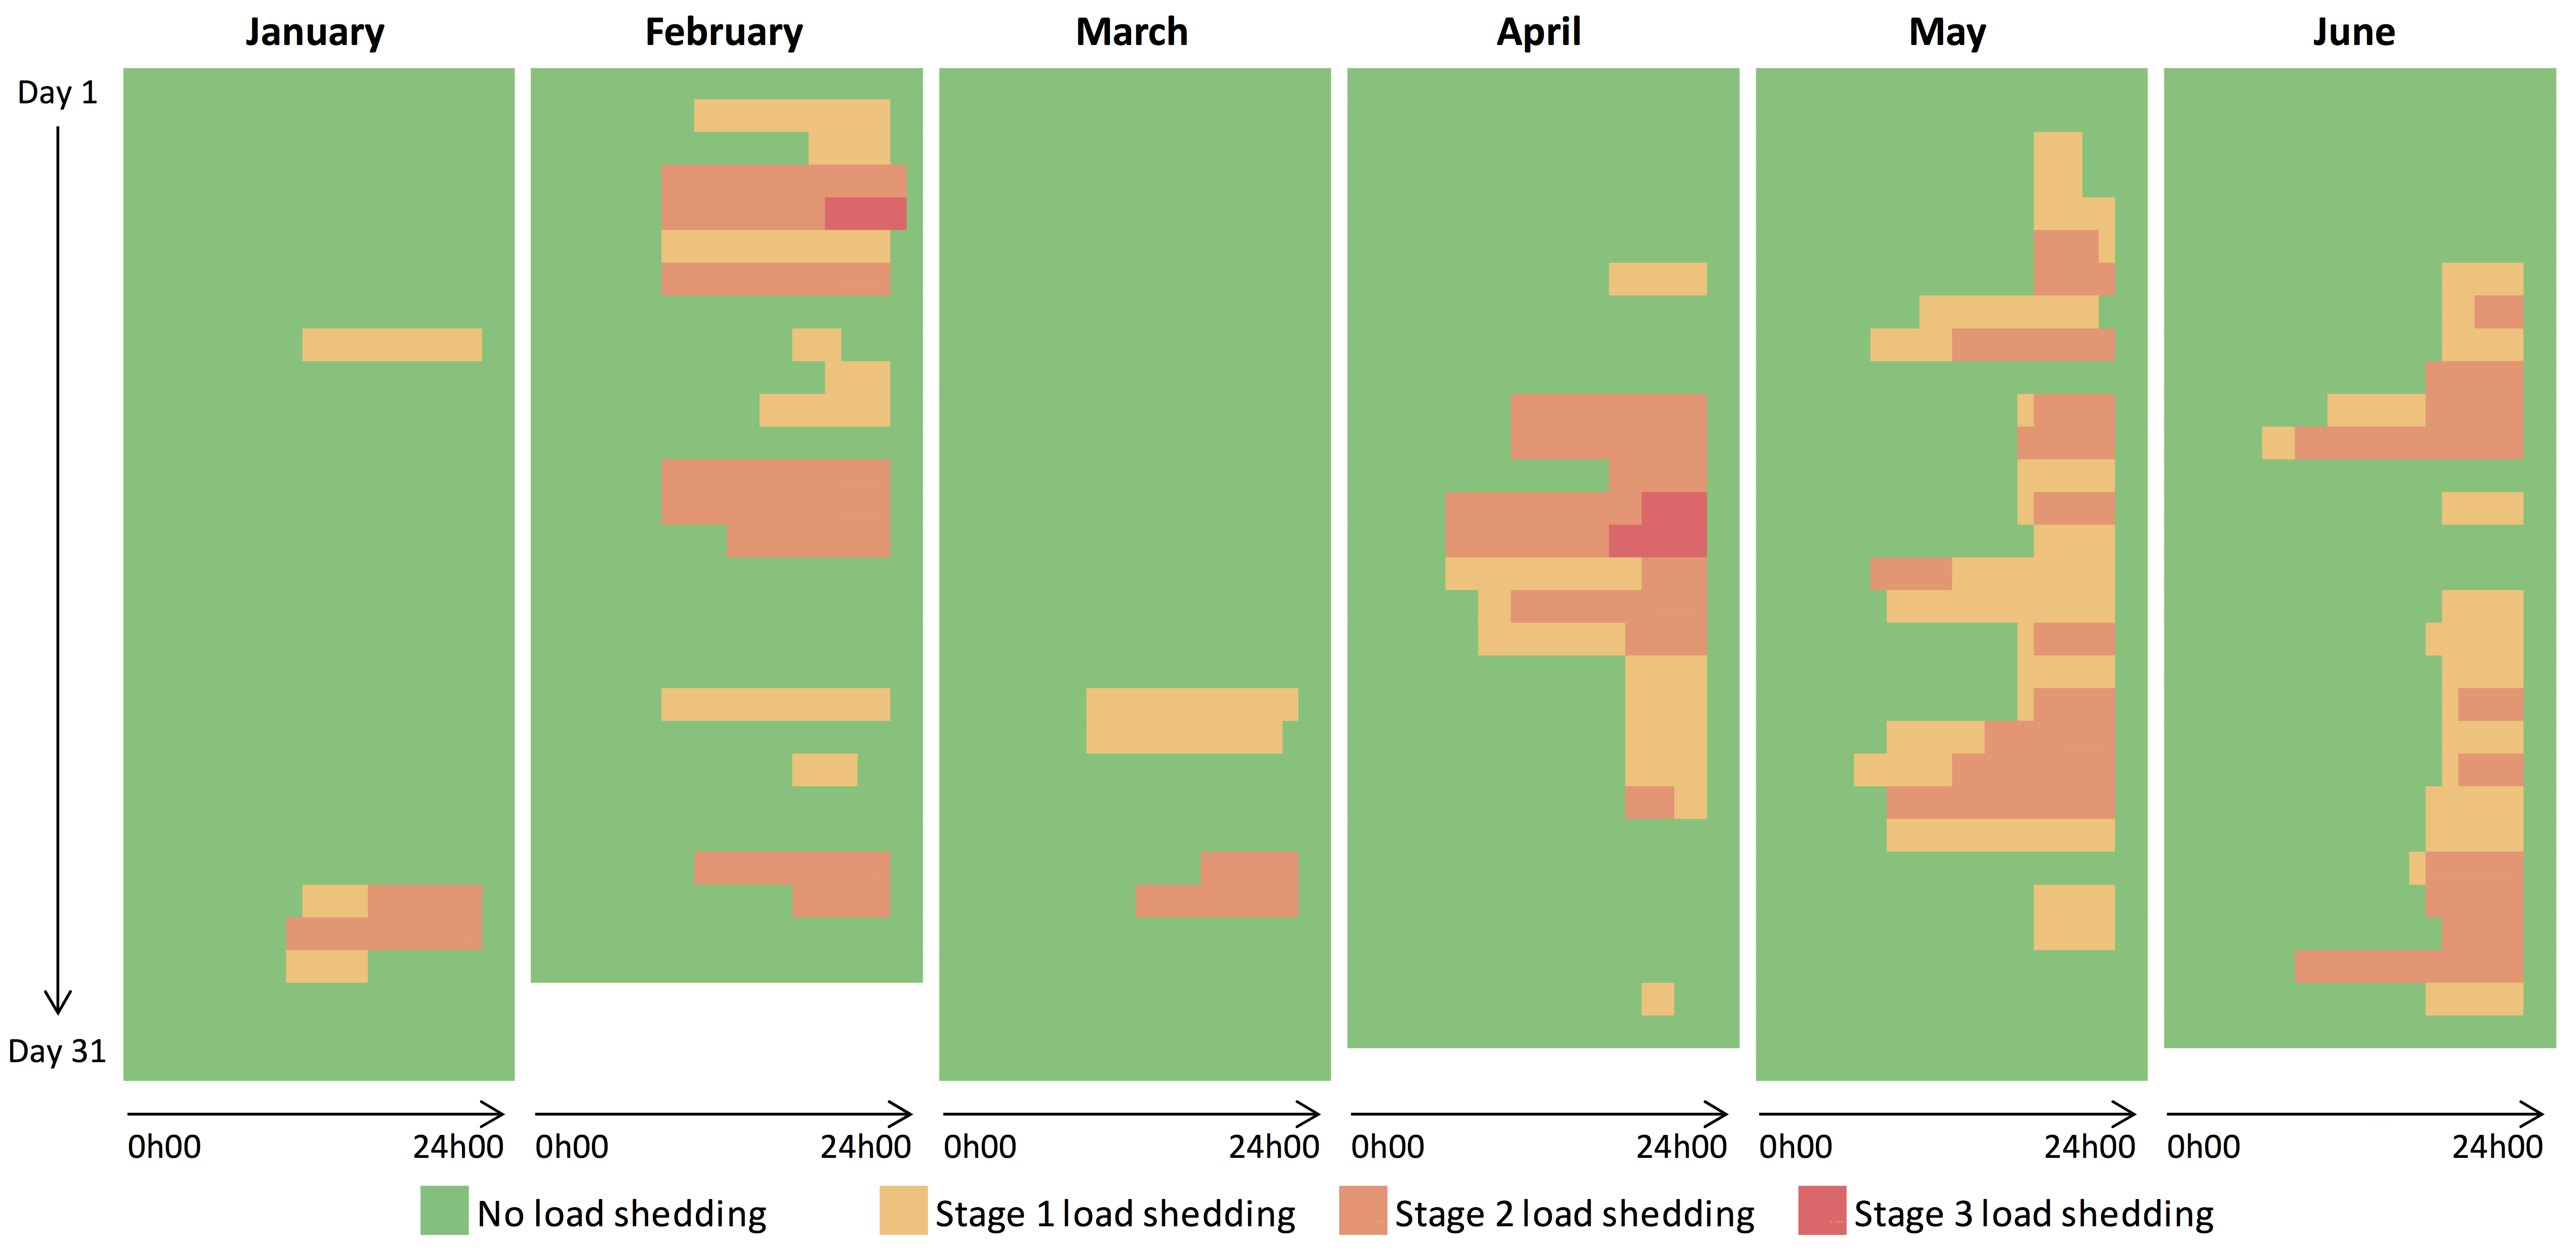
\includegraphics[width=1\linewidth]{FIG/Load_shedding}
\caption[Hourly distribution of load shedding from January to June 2015.]{Hourly distribution of actual load shedding from January to June 2015 \cite{CSIREnergyCentre2015}.}\label{Load_shedding}
\end{figure}

%SA has currently a total nominal installed capacity of \SI{45699}{\mega\watt}, therefrom Eskom owns and manage \SI{42090}{\mega\watt} power station capacity in March 2015 \cite{Eskom2015b}. Almost \SI{85}{\percent} of Eskom's power plant capacity are coal-fired (\SI{35721}{\mega\watt}), \SI{4.4}{\percent} nuclear (\SI{1860}{\mega\watt}) and \SI{5.7}{\percent} gas-fired (\SI{2409}{\mega\watt}) which is shown in Figure~\ref{PgenerationEskom}. Besides these fossil and nuclear based capacities Eskom owns also capacities in pumped storage (\SI{1400}{\mega\watt}), hydro (\SI{600}{\mega\watt}) and wind (\SI{100}{\mega\watt}). Further \SI{3609}{\mega\watt} capacity coming from independent power producers (IPP) which also include \SI{1795}{\mega\watt} renewable generation trough the Renewable Energy Independent Power Producer Procurement Program (REIPPPP). \cite{Eskom2015a}

South Africa currently has total nominal installed capacity of \SI{45699}{\mega\watt}, of which Eskom owns and manages \SI{42090}{\mega\watt} \cite{Eskom2015b}. Almost \SI{85}{\percent} of Eskom's capacity is provided by coal-fired plants (\SI{35721}{\mega\watt}), \SI{4.4}{\percent} by nuclear (\SI{1860}{\mega\watt}) and \SI{5.7}{\percent} natural gas-fired (\SI{2409}{\mega\watt}) (Figure~\ref{PgenerationEskom}). Eskom also owns pumped storage (\SI{1400}{\mega\watt}), hydroelectric (\SI{600}{\mega\watt}) and wind generating stations (\SI{100}{\mega\watt}). An additional \SI{3609}{\mega\watt} of capacity is provided by independent power producers (IPP), which includes \SI{1795}{\mega\watt} renewable generation through the Renewable Energy Independent Power Producer Procurement Program (REIPPPP) \cite{Eskom2015a}.

\begin{figure}[htbp]  
\centering
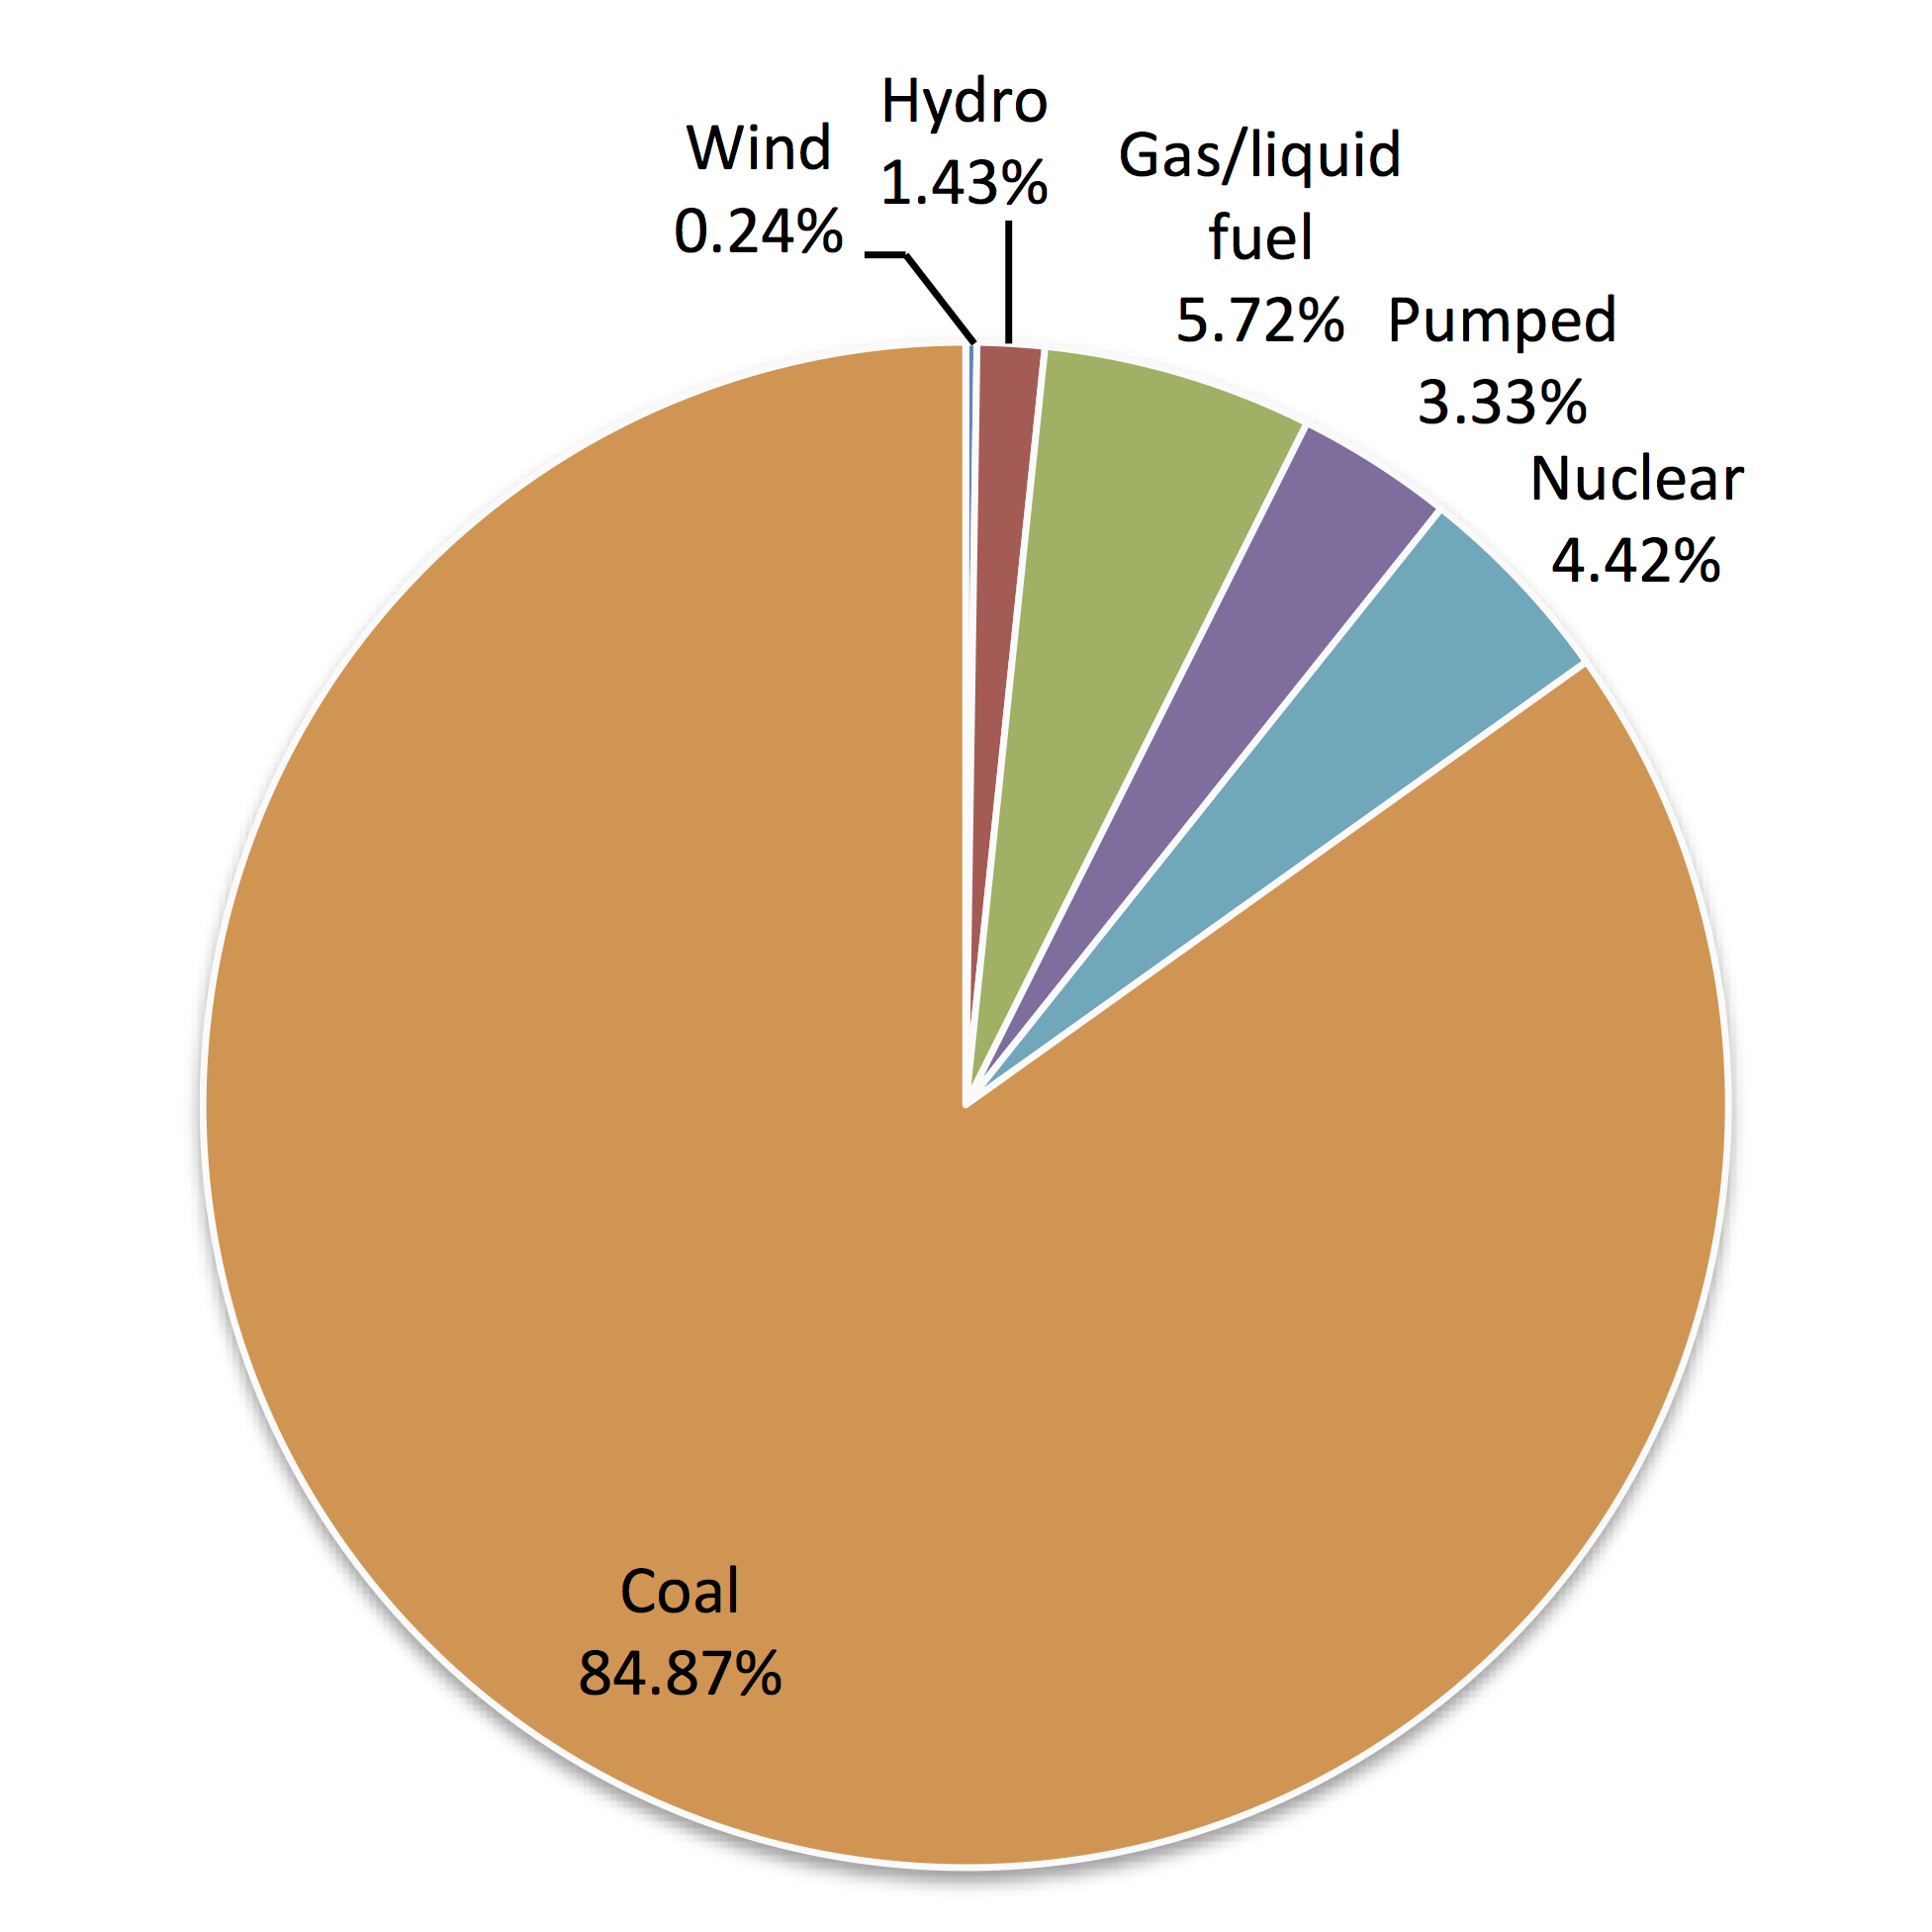
\includegraphics[width=0.45\linewidth]{FIG/Pgenerationeskom}
\caption[Eskom's nominal installed power station capacity in 2015.]{Eskom's nominal installed power station capacity in 2015 \cite{Eskom2015a}.}\label{PgenerationEskom}
\end{figure}
%The REIPPPP is one of the instruments that the SA Government uses to reaching there ambitious set target for a total installed capacity of \SI{81350}{\mega\watt} in 2030. From the aspired goal \SI{17430}{\mega\watt} are planed from wind and solar power. More precisely \SI{9770}{\mega\watt} by PV and \SI{3300}{\mega\watt} by CSP. \cite{DoE2013}
%
%After five bid windows (incl. extended bid window in March 2014) the REIPPPP reached a committed capacity of \SI{5237}{\mega\watt} wherefrome \SI{1899}{\mega\watt} are commited to PV and \SI{600}{\mega\watt} to CSP. \cite{DoE2015}
The REIPPPP is one of the instruments that the South African government is using to reach an ambitious target for total installed capacity of \SI{81350}{\mega\watt} by 2030. Of this, fully \SI{17430}{\mega\watt} are to come from wind and solar power (\SI{9770}{\mega\watt} from PV and \SI{3300}{\mega\watt} from CSP) \cite{DoE2013}.

After five bid windows (including an extended bid window in March 2014) the REIPPPP reached a committed capacity of \SI{5237}{\mega\watt} of which \SI{1899}{\mega\watt} are PV and \SI{600}{\mega\watt} are CSP \cite{DoE2015}.

%SA is a country of wide open spaces and cities and towns are separated by large distance. Therefore long transmission lines are needed to transport electricity from the large power plants of the Gauteng province to the coastal areas. Figure~\ref{transmissionprojekts} gives an overview of the current situation of the allocations of the power stations and the transmission lines. Also Eskoms future transmission and power station projects are featured in the figure.

Much of the existing power generation is located in the northeast, in Gauteng, the country's economic and industrial heartland. South African cities and towns are separated by large distances and long transmission lines are needed to transport electricity from the large power plants of Gauteng to the coastal areas (Figure~\ref{transmissionprojekts}). 

\begin{figure}[htbp]
\centering
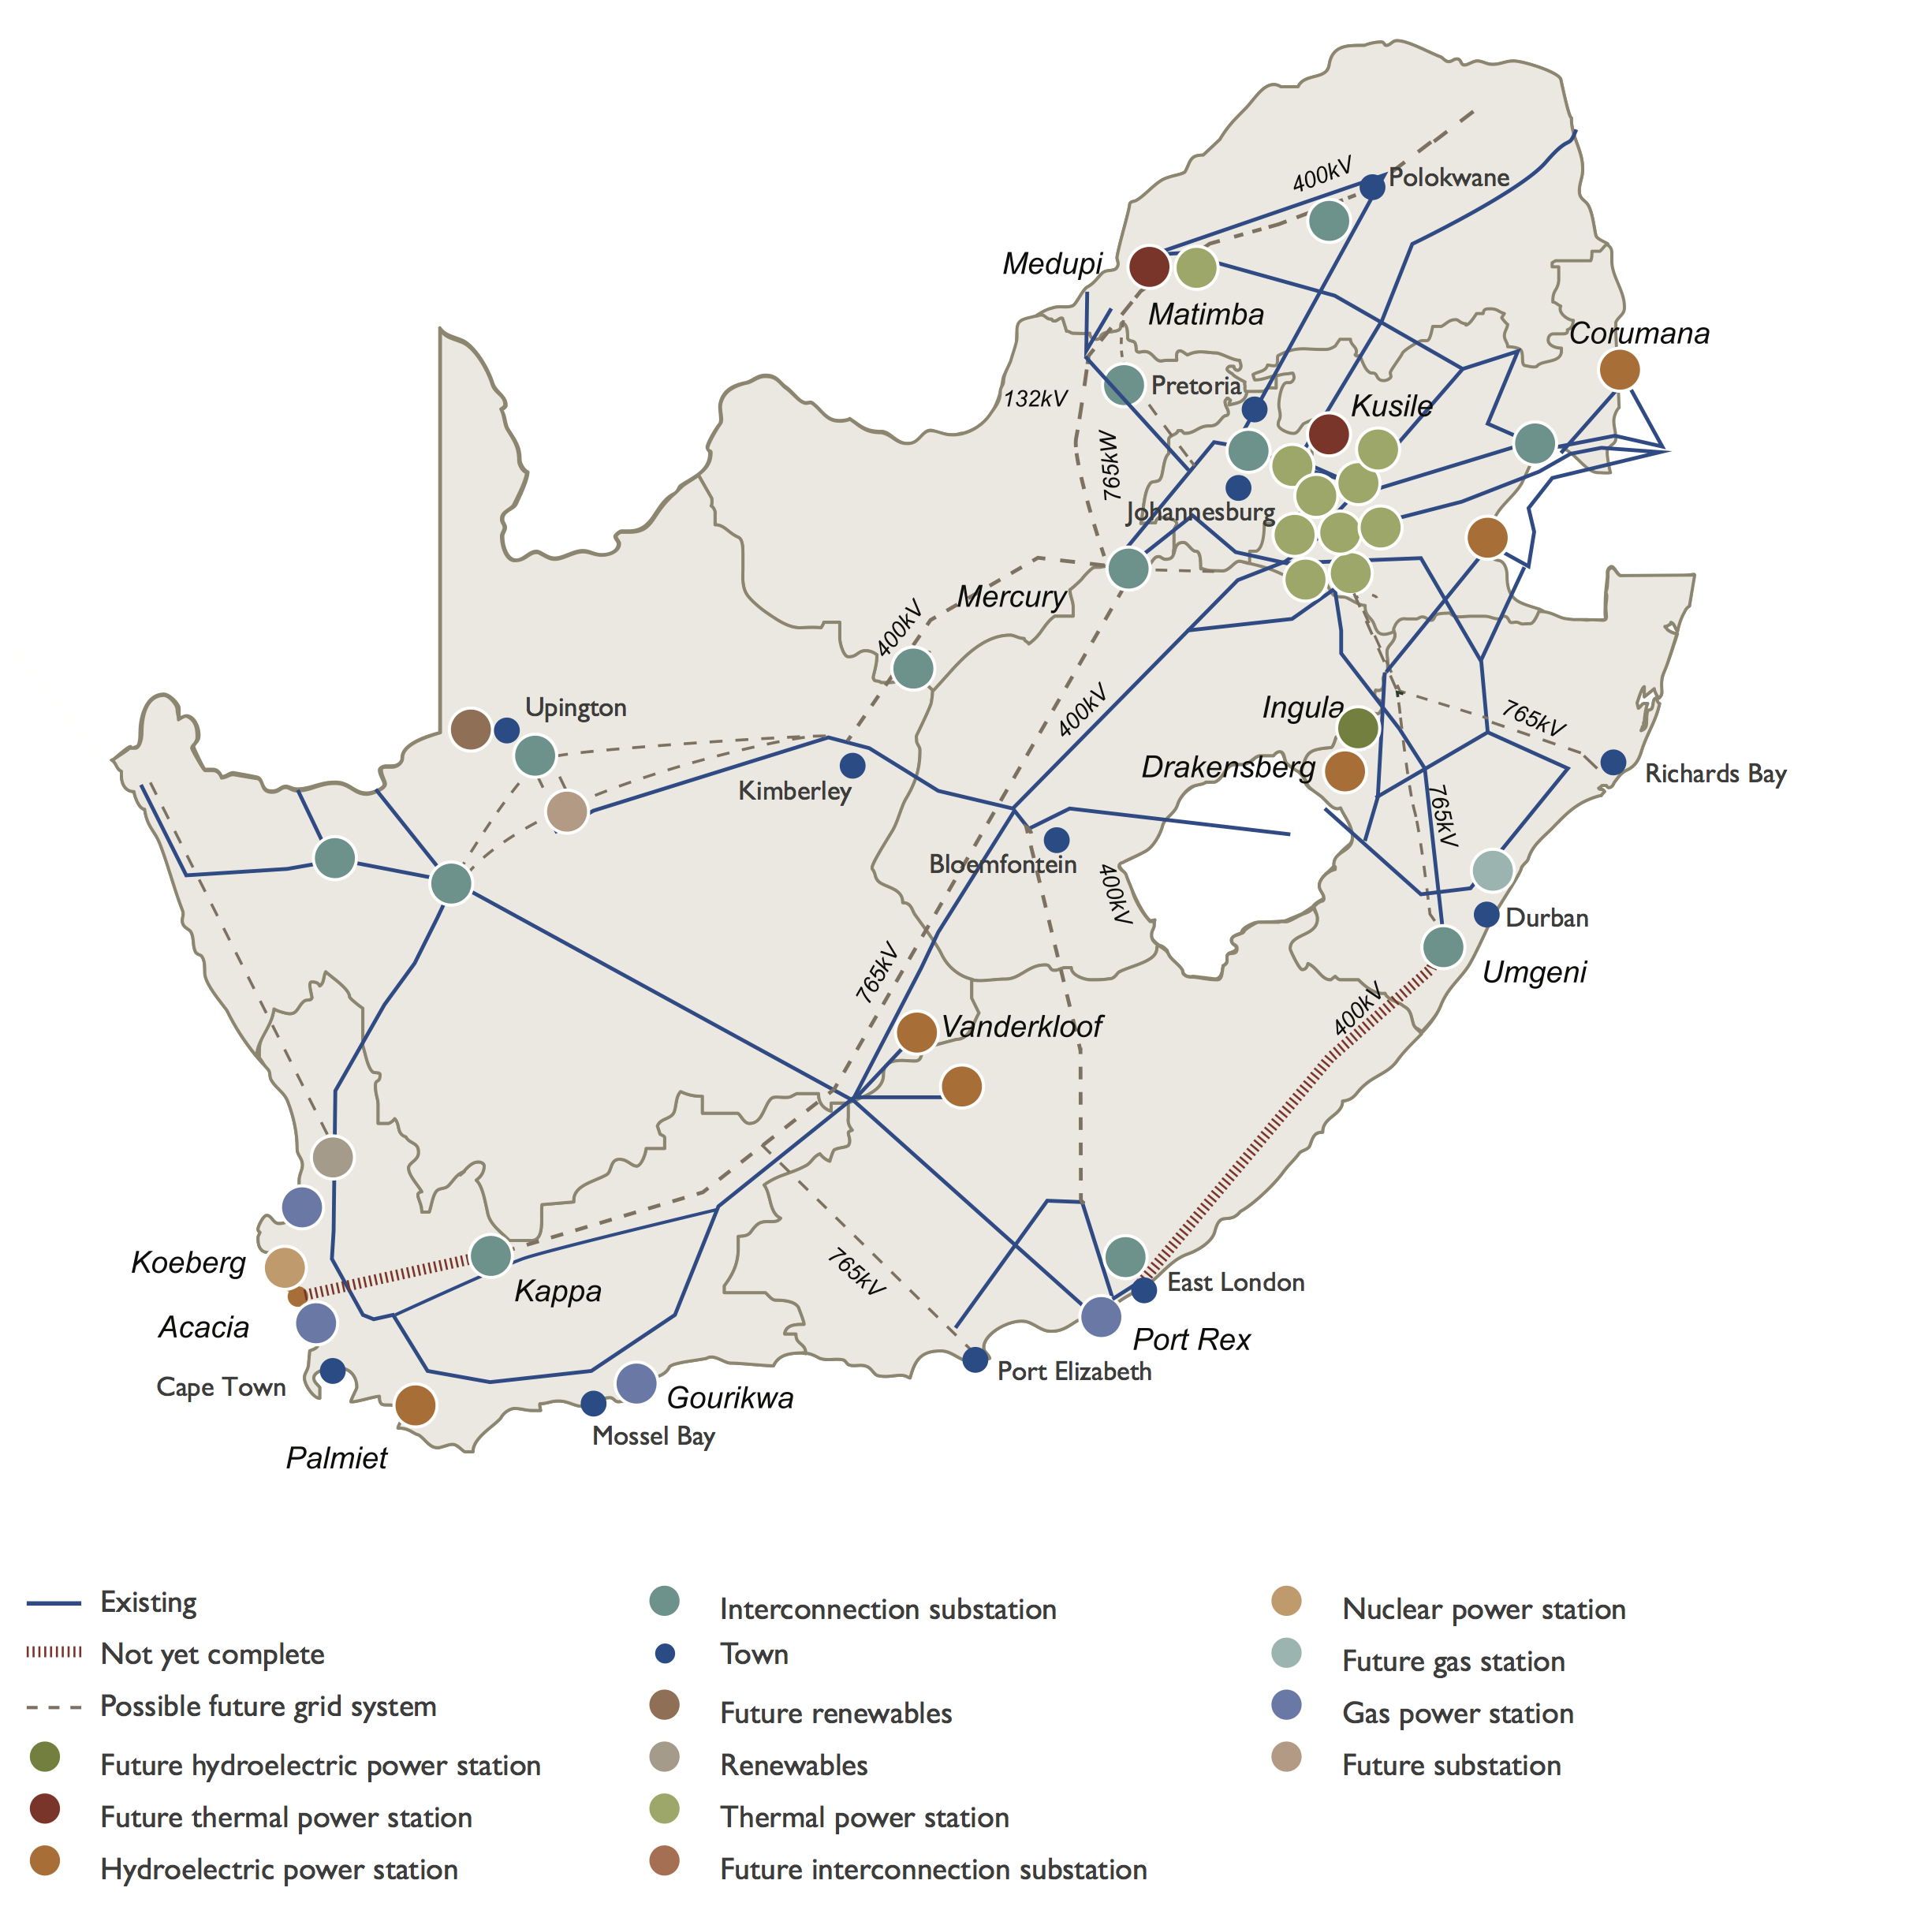
\includegraphics[width=1\linewidth]{FIG/transmissionprojekts}
\caption[Eskom’s transmission projects as at 31 March 2015.]{Eskom’s transmission projects as at 31 March 2015 \cite{Eskom2015a}.}\label{transmissionprojekts}
\end{figure}
%Eskom operates, manages and maintains a total distance of \SI{368331}{\kilo\meter} power lines, whereof \SI{31107}{\kilo\meter} are transmission power lines at \SIrange{765}{132}{\kilo\volt} and \SI{48278}{\kilo\meter} are distribution power lines at \SIrange{132}{33}{\kilo\volt}. The residual power lines are \SI{281510}{\kilo\meter} reticulation power lines which are below \SI{22}{\kilo\volt} and \SI{7436}{\kilo\meter} underground cables. Thereby is the country's total transformer capacity \SI{239490}{\mega\volt\ampere}. The whole power supply system is controlled to a frequency of \SI{50}{\hertz}. \cite{Eskom2015b}
Eskom operates, manages and maintains \SI{368331}{\kilo\meter} of power lines, of which \SI{31107}{\kilo\meter} are transmission lines at \SIrange{132}{765}{\kilo\volt} and \SI{48278}{\kilo\meter} are distribution power lines at \SIrange{33}{132}{\kilo\volt}. Of the residual power lines, \SI{281510}{\kilo\meter} are reticulation lines under \SI{22}{\kilo\volt} and \SI{7436}{\kilo\meter} are underground cables. The total transformer capacity is \SI{239490}{\mega\volt\ampere}. Grid frequency is \SI{50}{\hertz} \cite{Eskom2015b}.

%When taking again an eye on Figure~\ref{transmissionprojekts} it can be noted, that the area of Upington in the Northern Cape province is not yet accessed with high voltage transmission lines. Considering that the area of Upington provides the country’s highest solar irradiation value and is therefore a highly attractive site for solar power plants, new high voltage transmission lines to regions with higher load factors are necessary and are currently in its planning phase. Eskom is currently planing additional \SI{3940}{\kilo\meter} transmission lines and \SI{12815}{\mega\volt\ampere} transformer capacities till 2021 \cite{Eskom2015a}.

The region around Upington in the Northern Cape province is not connected to high voltage transmission lines (Figure~\ref{transmissionprojekts}). Because the region has the country's highest solar irradiation value and is therefore a highly attractive site for solar power plants, new high voltage transmission lines to regions with higher load factors are necessary and are currently in the planning phase. Eskom is planning to build an additional \SI{3940}{\kilo\meter} of transmission line and add \SI{12815}{\mega\volt\ampere} transformer capacity by 2021 \cite{Eskom2015a}.

%Through this electricity network SA covers a electrification rate of around \SI{85}{\percent} and which is the highest on mainland sub-Saharan Africa. About \SI{11}{\percent} of households don't have access to electricity and a further \SI{4}{\percent} rely on illegal access (non-paying) or obtain access informally (from one household to another but paying). \cite{IEA2014f}
This electricity network gives South Africa an overall electrification rate of approximately \SI{85}{\percent}, the highest in mainland sub-Saharan Africa. Of the remainder, \SI{11}{\percent} still do not have access to electricity and a further \SI{4}{\percent} rely on illegal access (non-paying) or obtain access informally (from one household to another but paying) \cite{IEA2014f}.

%In the financial year 2014/15 Eskom sales about \SI{216274}{\giga\watt\hour}. The spread of the main customers is shown in Figure~\ref{ElectricityShare}. From this it appears that the Municipalities are Eskom's biggest consumers. But also the Industrial and Mining sector makes together a considerable part of \SI{38.6}{\percent} of the electricity consumption. The residential part of the electricity consumption was just about \SI{5.36}{\percent} and the commercial part was below \SI{5}{\percent}. The main part of the exported electricity with about \SI{70}{\percent} went to the neighboring country Mosambique and further \SI{10}{\percent} to Botswana. Namibia and Swaziland mades just 8 or \SI{7}{\percent} of the exported electricity. \cite{Eskom2015b}  
In the fiscal year 2014/15, Eskom sold \SI{216274}{\giga\watt\hour} of electrical energy. Municipalities are the largest consumers (Figure~\ref{ElectricityShare}), but the industrial and mining sectors are also significant customers (\SI{38.6}{\percent} of electricity consumption). Households consumed \SI{5.36}{\percent} and the commercial sector less than \SI{5}{\percent}. The greatest share of exported electricity (\SI{70}{\percent}) went to Mozambique and a further \SI{10}{\percent} to Botswana. Namibia and Swaziland, also immediate neighbours, make up just \SI{8}{\percent} or \SI{7}{\percent} of the exported electricity \cite{Eskom2015b}.
\begin{figure}[!h] 
\centering
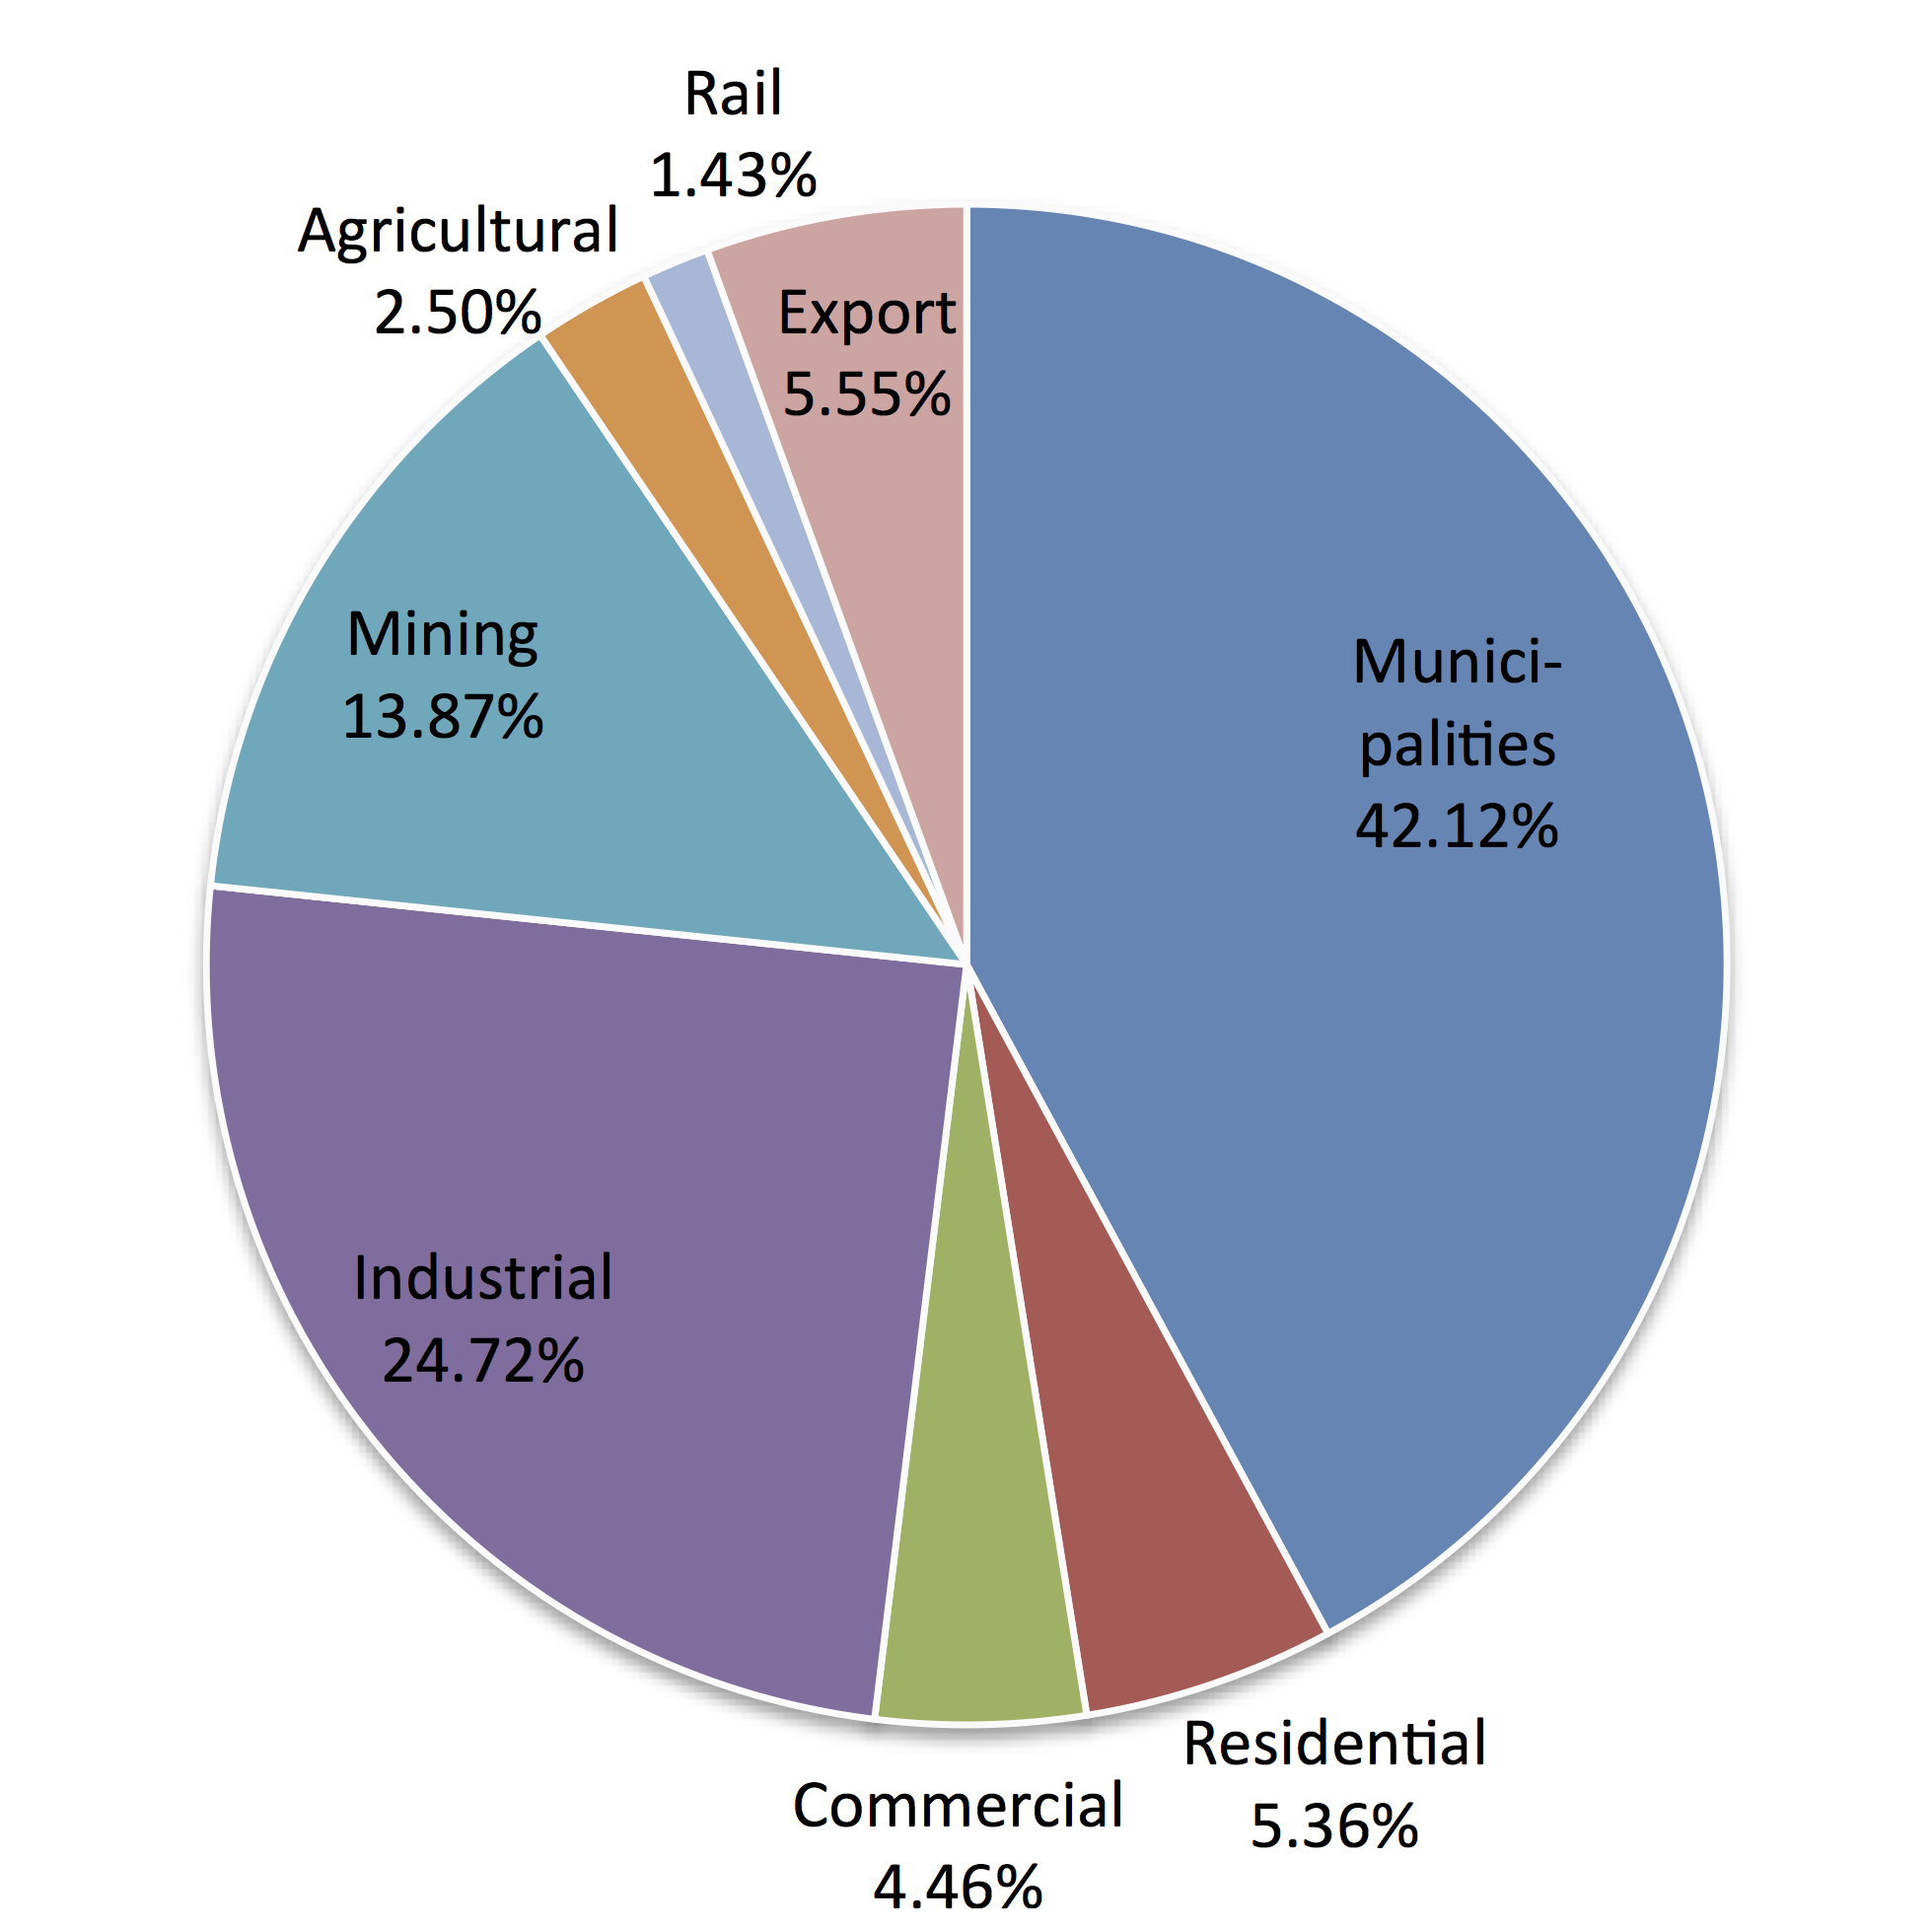
\includegraphics[width=0.5\linewidth]{FIG/ElectricityShare}
\caption[Eskom's electricity sales per customer category.]{Eskom's electricity sales per customer category \cite{Eskom2015b}.}\label{ElectricityShare}
\end{figure}
\pagebreak
